\documentclass[12pt,oneside,titlepage,letter]{article}

\usepackage[margin = 0.75in]{geometry} 

\setlength{\parindent}{0cm}



\usepackage[intlimits]{amsmath}  % AMS-Latex
\usepackage{amssymb}             % AMS-Latex
\usepackage{tikz}
\usepackage{ifthen}


\newcommand{\modify}[1]{{\color{blue}#1}}


\title{RnavGraph: an R package to visualize high dimensional data using graphs as navigational infrastructure}
\author{Adrian Waddell and Wayne Oldford}


\date{\today}

%\VignetteIndexEntry{Detailed manual to the RnavGraph package}
%\VignetteDepends{RnavGraph}
%\VignetteKeywords{navGraph}
%\VignettePackage{RnavGraph}
\usepackage{Sweave}
\begin{document}

\maketitle

\tableofcontents

\newpage
%\begin{center}
%{\Huge {\bf RnavGraph} -- Navigating dimensional data}
%\end{center}
\section{Introduction}
\texttt{RnavGraph} provides interactive visualization tools for exploring high dimensional space through lower dimensional trajectories, based on the concepts first presented in Hurley and Oldford (2011).  

\subsection{Getting started}
The \texttt{RnavGraph}  package is available from the Comprehensive R Archive Network (CRAN). We used extensively S4 classes and the Tcl and Tk API via the \texttt{tcltk} R package. Most of the visualization, both for the graph and the 2d scatterplots, build upon the Tk canvas widget.\\

\texttt{RnavGraph} depends on the packages: \texttt{methods}, \texttt{graphics}, \texttt{tcltk}, \texttt{graph} and \texttt{RBGL}. However to be able to run all demos and examples we suggest to install the following packages: \texttt{Rgraphviz}, \texttt{PairViz}, \texttt{scagnostics}, \texttt{rgl}, \texttt{grid}, \texttt{MASS}, \texttt{hexbin}, \texttt{RDRToolbox} and, optionally, \texttt{rggobi}.   These packages are available through the CRAN and/or Bioconductor R repositories. \\

Linux users should make sure that \texttt{tcl} and \texttt{tk} are installed. Further the package needs the following libraries (on a Ubuntu 10.04 system): \texttt{libtk-img}, \texttt{libtk-img-dev}, \texttt{tcl-dev} and \texttt{tk-dev}.\\

Once the package and all of its dependencies have been installed,  \texttt{RnavGraph} is loaded using
\begin{Schunk}
\begin{Sinput}
> library(RnavGraph)
\end{Sinput}
\end{Schunk}
A closer look into \texttt{RnavGraph} reveals that a relatively large set of functions are available that provide a programmable user interface to the package.
\begin{Schunk}
\begin{Sinput}
> ls("package:RnavGraph")
\end{Sinput}
\begin{Soutput}
 [1] "completegraph"       "linegraph"           "navGraph"           
 [4] "newgraph"            "ng_2d"               "ng_2d_ggobi"        
 [7] "ng_2d_myplot"        "ng_data"             "ng_get"             
[10] "ng_graph"            "ng_image_array_gray" "ng_image_files"     
[13] "ng_set"              "ng_set<-"            "ng_update"          
[16] "ng_walk"             "plot"                "scagEdgeWeights"    
[19] "scagGraph"           "scagNav"             "shortnames"         
[22] "shortnames<-"       
\end{Soutput}
\end{Schunk}

We try to explain all these functions within this vignette, though the R \texttt{help} function should also be used to get a more detailed description on any particular function, as needed. 
In addition, we provide the \texttt{RnavGraph} package with several demos that may be helpful, via
\begin{Schunk}
\begin{Sinput}
> demo(package = "RnavGraph")
\end{Sinput}
\end{Schunk}
The source code of these demos can be found in the system directory shown in the output from
\begin{Schunk}
\begin{Sinput}
> system.file("demo", package = "RnavGraph")
\end{Sinput}
\end{Schunk}
Many of the demos require data from the \texttt{RnavGraphImageData} package also written by us.\\

All said, though, this vignette should itself provide the best introduction to \texttt{RnavGraph} and its full functionality.
\subsection{A simple example}
We start with a simple example, using the famous Anderson Iris data, to quickly introduce the
basic functionality of \texttt{RnavGraph} and to give you a feel for its interface.
To begin, then, execute the following in R:
\begin{Schunk}
\begin{Sinput}
> library(RnavGraph)
> ng.iris <- ng_data(name = "iris", data = iris[,1:4],
+                    shortnames = c('s.L', 's.W', 'p.L', 'p.W'),
+                    group = iris$Species,
+                    labels = substr(iris$Species,1,2))
\end{Sinput}
\end{Schunk}
As the name suggests, \texttt{ng\_data} sets up a ``navgraph'' or ``ng'' data object (more on this later). 
Its  \texttt{data} argument takes a \texttt{data.frame} identifying the numeric variables to be explored.  The Iris data consists of measurements of the \texttt{Sepal.Length}, \texttt{Sepal.Width}, \texttt{Petal.Length}, and  \texttt{Petal.Width} on $50$ flowers of each of three \texttt{Species} of Iris. (The above construction uses the argument \texttt{shortnames}, instead of the variable names, just to give more compact labelling in the subsequent displays.) \\

The Iris data provides a set of 150 points in a four-dimensional space; our objective is to visually explore the structure of this data.  To begin this exploration, we simply call \texttt{navGraph} on the prepared data.
\begin{Schunk}
\begin{Sinput}
> navGraph(ng.iris)
\end{Sinput}
\end{Schunk}
Alternatively, if you have \texttt{rggobi} working in R and would like to visualize the data via \texttt{ggobi}, call
\begin{Schunk}
\begin{Sinput}
> navGraph(ng.iris, settings = list(defaultDisplay = "ggobi"))
\end{Sinput}
\end{Schunk}
Either of these calls will produce a {\em navigation graph} (or {\em navgraph} for short) as shown in
Figure \ref{fig:session1}(a)


\begin{figure}[h]   
  \centering
  \begin{tabular}{cc}
  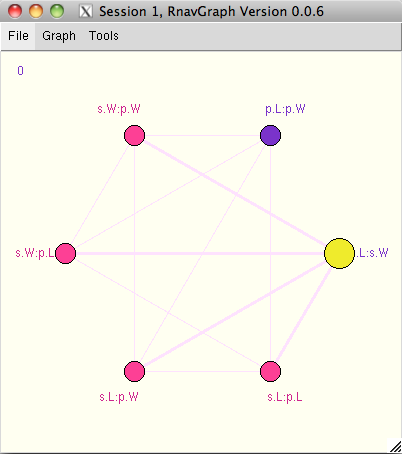
\includegraphics[width = 2.0in]{img/Iris3Dgraph.png} &
  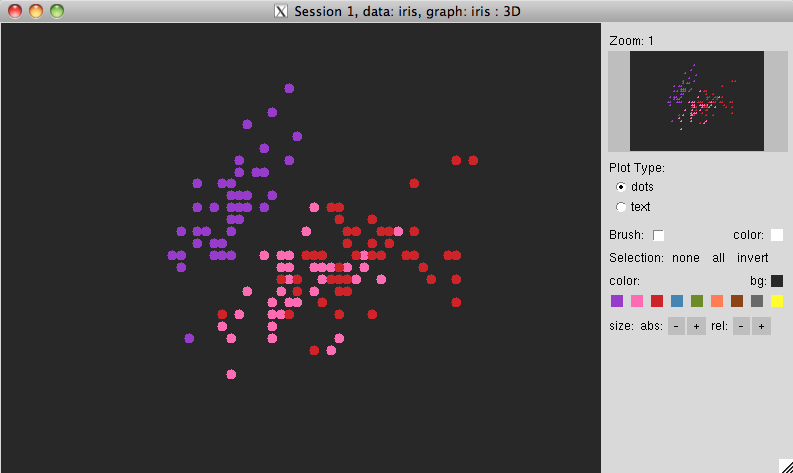
\includegraphics[width = 4in]{img/Iris2D.png} \\
  {\small (a) The 3D transition graph}&
  {\small (b) The associated display: 2D plot}\\
  \end{tabular}
  \caption{navGraph on the Anderson Iris data.}
\label{fig:session1}
\end{figure}
and a ``visualization'' such as that of Figure  \ref{fig:session1}(b).
Here, Figure  \ref{fig:session1}(b) is a \texttt{2D} display, native to \texttt{navGraph}, as produced by the first of the above \texttt{navGraph} calls (the second call would produce a \texttt{ggobi} session instead).   
The variates \texttt{Sepal.Length} and \texttt{Sepal.Width} determine the coordinates of the points in the scatterplot and the \texttt{group}, here  \texttt{Iris\$Species}, determine the point colours.  
If you select ``text'' in the  \texttt{2D} plot, the point symbols will be replaced by the text strings
identified by the \texttt{labels} argument in the definition of the ``ng data'' \texttt{ng.iris}.\\

The graph of Figure \ref{fig:session1}(a), the {\em navigation graph}, is programmatically linked to the \texttt{2D plot} data visualization of Figure \ref{fig:session1}(b).
The large yellow circle on the rightmost node of the graph is called the ``bullet''; its position in the graph represents a well-defined location in the high-dimensional data space which, in turn, determines what is actually displayed in the visualization of Figure \ref{fig:session1}(b).  In Figure \ref{fig:session1}(a), it sits on a node labelled \texttt{s.L:s.W} and so Figure \ref{fig:session1}(b) displays a scatterplot for the variates  \texttt{Sepal.Length} and \texttt{Sepal.Width} (``shortnames'' being \texttt{s.L} and \texttt{s.W}, respectively).\\

Note how the other nodes are coloured differently, and the edges to them highlighted, depending upon whether they share an edge with the bullet's current node or not.  
You can move the bullet to a connected node simply by double-clicking on the destination node, by selecting the destination node and scrolling, or by simply selecting and dragging the bullet itself.
However you choose to do so, the bullet will dynamically traverse the edge from origin to destination node while, at the same time, the scatterplot display
will ``follow'' the bullet's path smoothly updating its display.\\

Try it, moving the bullet from the original node \texttt{s.L:s.W} to the upper left node \texttt{s.W:p.W}.
The effect in the scatterplot will be that of rotating the \texttt{s.L} axis into that of the \texttt{p.W} axis.
The shared variate, \texttt{s.W} will remain in place.  \\

Now make a number of connected moves in sequence along the graph.  
As you move the bullet along a path, the scatterplot will continually update via rigid rotations.
Note also that each time the bullet arrives at a new node, its potential destination nodes and edges are highlighted anew, and those edges which have already been traversed are coloured slightly different from those which have not yet been visited.  Your connected sequence of edges constitutes a path on the navigation graph which, when followed by the bullet, causes the 2D display
to update, dynamically following various 3D trajectories through the four dimensional space
of the Iris data. \\

The effect is made more apparent by explicitly choosing the entire path in advance.  This is done using ``shift-select''.  Simply hold the shift-key down continuously and select each node (single-click) in turn along 
a path of your choice.  The path will be highlighted as you go.  Double-click for the final destination
and the bullet will immediately start to walk the path you have identified.  This will allow you to focus on the movement in the scatterplot display as the path is walked.\\

Having just walked a path, you might care to re-run it.  To do so, choose the ``Tools'' menu on the navgraph display and select the menu item ``Paths''.  A new window will open where the path just walked is recorded as the ``Active Path''.   This path may be viewed on the navgraph by pressing the ``view'' button, or walked again by pressing the ``walk'' button.  The active path may also be saved by pushing the ``save'' button and, once saved, made active again by double-clicking on the path in the list of saved paths.  It is also possible to select paths and type in comments related to the selected path.  In this way, the user can record interesting paths, describe the interesting features found, and walk them again at a later date.  Simply close the paths display when finished.\\

(The graphical user interface is described later in much more detail.)

\subsection{Underlying graph theory}
The graph theory underlying RnavGraph is given in detail in the paper by Hurley and Oldford (2011)
and we direct the reader there to gain a fuller appreciation.  In this section, we give only a brief summary of some of the ideas.\\

In the Iris example just considered, the nodes of Figure \ref{fig:session1}(a) are connected {\bf only if} they share a variate.  As a consequence of this, any travel along an edge is consistent with a
 a rigid rotation through a three dimensional subspace from one two-dimensional space (or scatterplot) to another.   Because the edges are restricted in this way, Hurley and Oldford (2011) call such a graph, a  {\em 3D transition graph}.\\

The {\em complement} of a 3D transition graph is the graph having the same nodes but with edges
appearing only between nodes that have {\bf no} variates in common.  That is only those edges missing between nodes in Figure \ref{fig:session1}(a) will appear in its complement.  Hurley and Oldford (2011) call this graph the corresponding {\em 4D transition graph}. \\

In our Iris example, choosing the ``Graph'' menu from the navgraph display of Figure \ref{fig:session1}(a) gives a menu of graphs to choose from.  Selecting the menu item ``iris: 4D'' will
cause the 4D transition graph to be displayed in place of the 3D transition graph and will also update the
scatterplot display.   \\

Since nodes no longer share a variable, moving the bullet along an edge in a
4D transition graph causes the 2D subspace (or scatterplot) at one node to smoothly transition
to the 2D subspace (or scatterplot) at the destination node.  This is effected by having both axes of one subspace simultaneously transformed into the axes of the other subspace along a geodesic in the four dimensional space defined by all 4 axes.   In this way, the path is essentially like that followed in \texttt{ggobi} but restricted to the four variates.  Walking a path on a 4D transition graph amounts to exploring the entire (possibly higher) dimensional space via four dimensional trajectories.\\

At this point, you might give the 4D transition a try.  You will see that the 4D transitions are not rigid rotations and so might look a little unnatural.\\

Hurley and Oldford (2011) describe a variety of ways to construct meaningful 3D and 4D transition graphs.  Fundamentally, these all begin with a graph on the variates themselves.\\

Hurley and Oldford (2011) define a variable graph $G$ as any graph, whose nodes are variates, and whose edges indicate an interest (however defined) in the pair of variates each edge joins in the graph $G$.\\

For example, if we consider again the Iris data with $p=4$ variates and assume that all pairs of variates are of equal interest, then $G$ could be the {\em complete graph} on four variates given by
the leftmost graph of Figure \ref{LLGLGNOT} (where \textit{A = Sepal.Length, B = Sepal.Width, C = Petal.Length, D = Petal.Width}).
\begin{figure}[h]
  \centering
  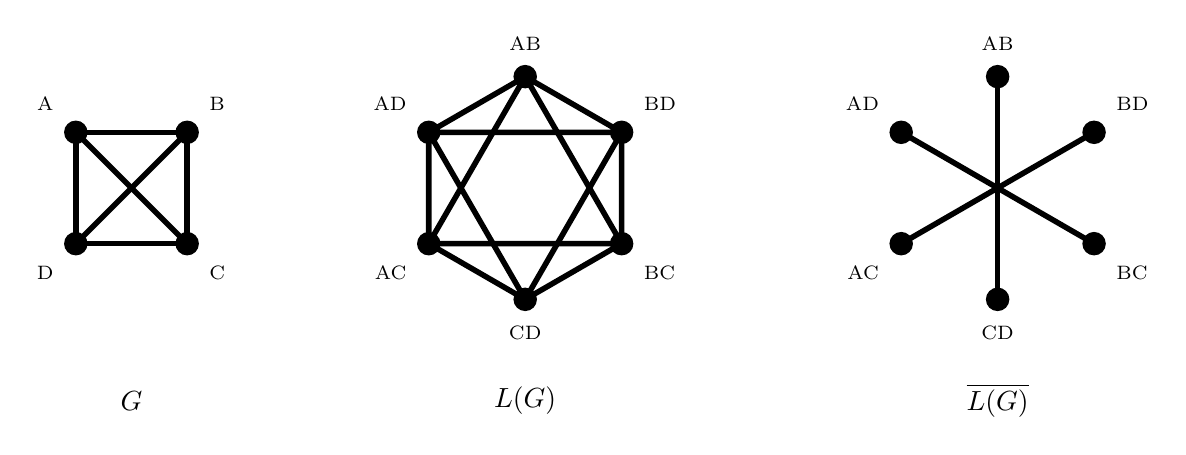
\begin{tikzpicture}
[node/.style={shape = circle, fill=black,inner sep = 3pt},
edge/.style={line width=2pt}]
\def\radius{1}
\begin{scope}
  \coordinate (A) at (135:\radius);
  \coordinate (B) at (45:\radius);
  \coordinate (C) at (-45:\radius);
  \coordinate (D) at (-135:\radius);
  
  \draw [-,edge] (A) -- (C);
    \draw [-,edge] (B) -- (D);
  \draw [-,edge] 
  (A) node [node,label=above left:{\scriptsize A}] {} -- 
  (B) node [node,label=above right:{\scriptsize B}] {} --
  (C) node [node,label=below right:{\scriptsize C}] {} --
  (D) node [node,label=below left:{\scriptsize D}] {} -- (A);

  \node at (0,-2.7) {$G$};
\end{scope}

\def\radius{1.414214}
\begin{scope}[shift={(5,0)}]
  \coordinate (AB) at (90:\radius);
  \coordinate (AD) at (150:\radius);
  \coordinate (AC) at (210:\radius);
  \coordinate (CD) at (270:\radius);
  \coordinate (BC) at (330:\radius);
  \coordinate (BD) at (30:\radius);  

  \draw [-,edge] (AD) -- (BD) -- (CD) -- cycle;
  \draw [-,edge] (AB) -- (AC) -- (BC) -- cycle;
  \draw [-,edge] 
  (AB) node [node,label=above:{\scriptsize AB}] {} -- 
  (AD) node [node,label=above left:{\scriptsize AD}] {} --
  (AC) node [node,label=below left:{\scriptsize AC}] {} --
  (CD) node [node,label=below:{\scriptsize CD}] {} -- 
  (BC) node [node,label=below right:{\scriptsize BC}] {} -- 
  (BD) node [node,label=above right:{\scriptsize BD}] {} -- (AB);
  \node at (0,-2.7) {$L(G)$};
\end{scope}


\def\radius{1.414214}
\begin{scope}[shift={(11,0)}]
  \coordinate (AB) at (90:\radius);
  \coordinate (AD) at (150:\radius);
  \coordinate (AC) at (210:\radius);
  \coordinate (CD) at (270:\radius);
  \coordinate (BC) at (330:\radius);
  \coordinate (BD) at (30:\radius);  

  \draw [-,edge] 
  (AB) node [node,label=above:{\scriptsize AB}] {} -- 
  (CD) node [node,label=below:{\scriptsize CD}] {};
  \draw [-,edge] 
  (AD) node [node,label=above left:{\scriptsize AD}] {} --
  (BC) node [node,label=below right:{\scriptsize BC}] {};
  \draw [-,edge] 
  (AC) node [node,label=below left:{\scriptsize AC}] {} --
  (BD) node [node,label=above right:{\scriptsize BD}] {};
  \node at (0,-2.7) {$\overline{L(G)}$};
\end{scope}


\end{tikzpicture}




% 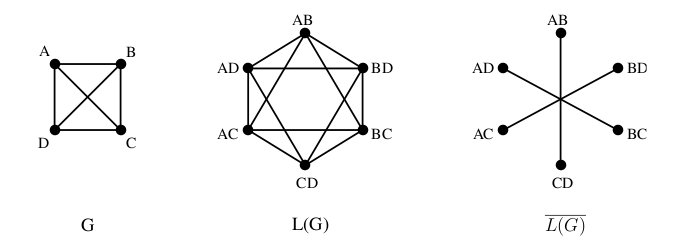
\includegraphics[width = 0.9 \textwidth]{lg.jpg}
  \caption{Complete graph $G$ with the individual variables as nodes. Line graph $L(G)$ which is equivalent to the 3d-transition graph. $\overline{L(G)}$ the 4d transition graph.}
  \label{LLGLGNOT}
\end{figure}
\\

A handy constructor from graph theory is the {\em line graph} of a graph $G$ denoted by $L(G)$.
This and other constructors are given in detail in Hurley and Oldford (2011).  Suffice to say here is that every edge in $G$ becomes a node in $L(G)$ and nodes in $L(G)$ have edges between them if and only if the corresponding edges in $G$ meet at a node in $G$.
For our purposes, it is enough to know that $L(G)$ will be a 3D transition graph, whatever the graph $G$ (provided it is a variable graph).  Moreover, the complement of $L(G)$ will be a 4D transition graph.  These three graphs are shown for the Iris data in Figure \ref{LLGLGNOT}.\\

Another means of constructing 3D and 4D transition graphs given by Hurley and Oldford (2011) is the use of various {\em graph products}.
If the variables --from the data-- separate into two sets, say $\mathcal{U} = \{U_1,U_2,...,U_m\}$ and $\mathcal{V} = \{V_1,V_2,...,V_n\}$, and for each set there is a corresponding variable graph which connects the pairs of interest, then the {\em Cartesian product} of the two graphs will produce a 3D transition graph preserving the pairs of interest and its complement, the {\em tensor product} on graphs will be the corresponding 4D transition graph.
Figure \ref{fig:prduct} shows these, and other, graph products.
\begin{figure}[h]
  \begin{tiny}
    \begin{center}
      %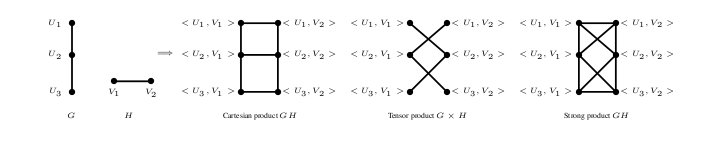
\includegraphics[width =  \textwidth]{products.jpg}
      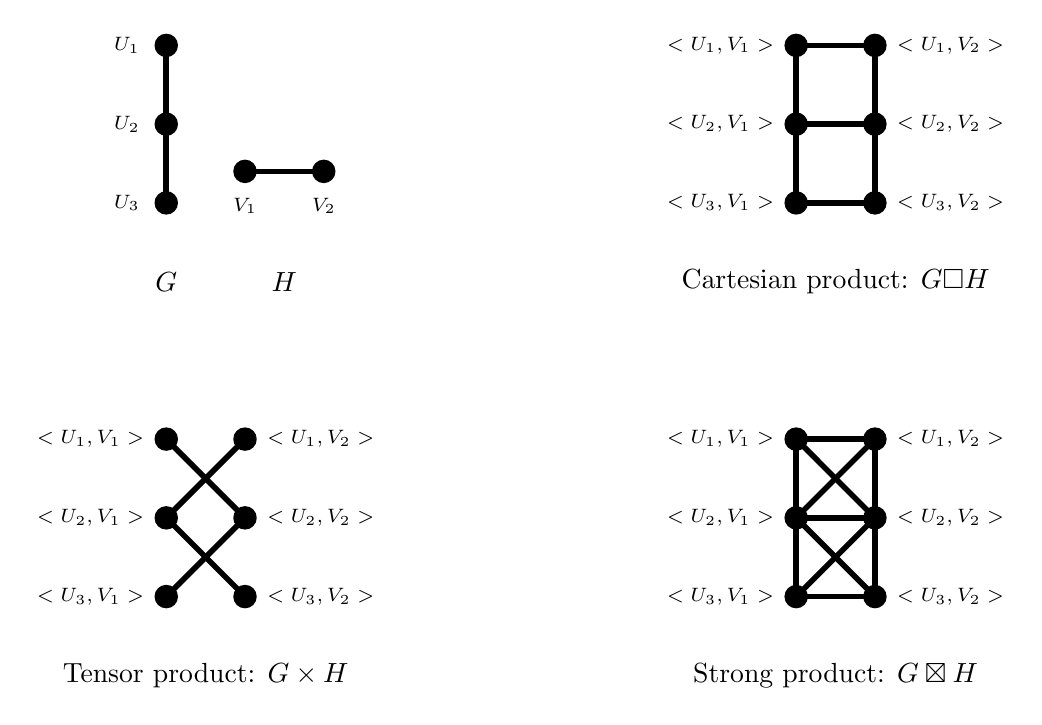
\begin{tikzpicture}
  [node/.style={shape = circle, fill=black,inner sep = 3pt},
edge/.style={line width=2pt}]

\begin{scope}
  \coordinate (U1) at (0,2);
  \coordinate (U2) at (0,1);
  \coordinate (U3) at (0,0);
  \coordinate (V1) at (1,0.4);
  \coordinate (V2) at (2,0.4);

 \draw [-,edge] 
  (U1) node [node,label=left:{\scriptsize $U_1$}] {} --
  (U2) node [node,label=left:{\scriptsize $U_2$}] {} --
  (U3) node [node,label=left:{\scriptsize $U_3$}] {};
  
 \draw [-,edge] 
  (V1) node [node,label=below:{\scriptsize $V_1$}] {} --
  (V2) node [node,label=below:{\scriptsize $V_2$}] {};  

\node at (0,-1) {$G$};
\node at (1.5,-1) {$H$};
\end{scope}


\newcommand{\GP}{
  \coordinate (U1V1) at (0,2);
  \coordinate (U2V1) at (0,1);
  \coordinate (U3V1) at (0,0);
  \coordinate (U1V2) at (1,2);
  \coordinate (U2V2) at (1,1);
  \coordinate (U3V2) at (1,0);
  
  \node at (U1V1) [node,label=left:{\scriptsize $<U_1,V_1>$}] {};
  \node at (U2V1) [node,label=left:{\scriptsize $<U_2,V_1>$}] {};
  \node at (U3V1) [node,label=left:{\scriptsize $<U_3,V_1>$}] {};
  \node at (U1V2) [node,label=right:{\scriptsize $<U_1,V_2>$}] {};
  \node at (U2V2) [node,label=right:{\scriptsize $<U_2,V_2>$}] {};
  \node at (U3V2) [node,label=right:{\scriptsize $<U_3,V_2>$}] {};
}
\begin{scope}[shift={(8,0)}]
  \GP

\draw [-,edge] (U1V1) -- (U3V1) -- (U3V2) -- (U1V2) -- cycle;
\draw [-,edge] (U2V1) -- (U2V2);

\node at (0.5,-1) {Cartesian product: $G \square H$};
\end{scope}

\begin{scope}[shift={(0,-5)}]
  \GP
\draw [-,edge] (U1V1) -- (U2V2) -- (U3V1);
\draw [-,edge] (U1V2) -- (U2V1) -- (U3V2);
  
\node at (0.5,-1) {Tensor product: $G\times H$};
\end{scope}


\begin{scope}[shift={(8,-5)}]
  \GP
\draw [-,edge] (U1V1) -- (U3V1) -- (U3V2) -- (U1V2) -- cycle;
\draw [-,edge] (U1V1) -- (U2V2) -- (U3V1);
\draw [-,edge] (U1V2) -- (U2V1) -- (U3V2);
\draw [-,edge] (U2V1) -- (U2V2);
\node at (0.5,-1) {Strong product: $G\boxtimes H$};
\end{scope}


\end{tikzpicture}

    \end{center}  
  \end{tiny}  
  \caption{Graph products}
  \label{fig:prduct}
\end{figure}
Although RnavGraph does not yet implement these products, it will in the next release.\\

Please see Hurley and Oldford (2011) for more details.

\subsection{General Structure of \texttt{RnavGraph} }
Before going further, it is important to realize that neither the underlying theory nor the implementation of \texttt{RnavGraph} presupposes that the only visualization of interest is that of
rotating scatterplots.\\

The theory, so far (though Hurley and Oldford, 2011, go beyond 2D nodes), only takes it that each
node of a transition graph represents 2D information of some sort and that an edge connects
two sets of 2D information which either share a single dimension (a 3D transition) or share no dimension (a 4D transition).  When imagining scatterplots at each node, it is easy to see that walking a path on the graph amounts to following a low dimensional trajectory through the higher dimensional space.\\

\texttt{RnavGraph} allows the user to define what visualization the vertices (or nodes) represent and what the transition (along the edges) represent.   Moreover, moving a bullet along  graph edge simply means updating the visualization with information on the current position between two nodes.
What a visualization chooses to do with such information depends entirely on the visualization.\\

The implementation of RnavGraph is general in that it makes no assumptions about either the views being displayed
or the nature of the transitions between them.  
\texttt{RnavGraph} integrates \textit{data to be analyzed}, \textit{a graph to navigate} and \textit{visualization instructions} to be executed as the graph is traversed. \\

\texttt{RnavGraph} provides an S4 class for each of these components to encapsulate the corresponding information, namely the classes \texttt{NG\_data}, \texttt{NG\_graph} and \texttt{NG\_Visualization}, respectively (their associated constructor functions will be explained later). The \texttt{navGraph()}  function in R takes  \texttt{graph}, \texttt{data} and \texttt{visualization} objects as arguments and starts up the corresponding graphical user interface. Figure \ref{fig:exampleSession} shows a stylized session.

\usetikzlibrary{calc}
\def\wi{0.8cm}
\pgfdeclareimage[width=\wi]{f1_1}{img/f1_1}
\pgfdeclareimage[width=\wi]{f1_2}{img/f1_2}
\pgfdeclareimage[width=\wi]{f2_1}{img/f2_1}
\pgfdeclareimage[width=\wi]{f2_2}{img/f2_2}
\pgfdeclareimage[width=\wi]{m1_1}{img/m1_1}
\pgfdeclareimage[width=\wi]{m1_2}{img/m1_2}
\pgfdeclareimage[width=\wi]{m2_1}{img/m2_1}
\pgfdeclareimage[width=\wi]{m3_1}{img/m3_1}
\pgfdeclareimage[width=\wi]{m4_1}{img/m4_1}
\pgfdeclareimage[width=\wi]{m4_2}{img/m4_2}


\begin{figure}[h]
\begin{center}
\begin{tikzpicture}
  [node/.style={circle, draw=black!50, fill=black!50, minimum size=3mm},
  bullet/.style={circle, draw=black, fill=black!10,thick, minimum size=6mm},
  notvisited/.style={draw=black},
  active/.style={draw=black!30,line width=4pt}]
  \begin{scope}
  \node at (-1, 0) [node, label=left:{\scriptsize A:D}] (N1) {};
  \node at ( 0,-1) [node, label=below:{\scriptsize B:C}] (N2) {};
  \node at ( 1, 0) [node, label=right:{\scriptsize C:D}] (N3) {};
  \node at ( 0, 1) [node, label=above:{\scriptsize A:B}] (N4) {};
  \draw[notvisited] (N3) -- (N2) -- (N1) -- (N4) -- (N2);
  \draw[active] (N3) -- (N1);
  \node at ( 0.4, 0) [bullet] {};  
  \draw (-2,-1.6) -- (2,-1.6) -- (2,1.6) -- (-2,1.6) -- (-2,-1.6);
  \node at (-2,1.8) [anchor=west] {interactive graph};
  \end{scope}
  
  
  %% 2d Scatterplot 
  \begin{scope}[shift={(4.4,0)}]
    \node at ( -0.8, -0.8) {\pgfbox[center,center]{\pgfuseimage{f1_1}}};
    \node at ( -0.2, -0.6) {\pgfbox[center,center]{\pgfuseimage{f1_2}}};
    \node at ( 2.6, 0.6) {\pgfbox[center,center]{\pgfuseimage{f2_1}}};
    \node at ( 3, -0.4) {\pgfbox[center,center]{\pgfuseimage{f2_2}}};
    \node at ( 1.6, 0.8) {\pgfbox[center,center]{\pgfuseimage{m1_1}}};
    \node at ( 1.0, 1) {\pgfbox[center,center]{\pgfuseimage{m1_2}}};
    \node at ( -1, 0.6) {\pgfbox[center,center]{\pgfuseimage{m2_1}}};
    \node at ( 0, 0.6) {\pgfbox[center,center]{\pgfuseimage{m3_1}}};
    \node at ( 1.2, -0.6) {\pgfbox[center,center]{\pgfuseimage{m4_1}}};
    \node at ( 2, -1) {\pgfbox[center,center]{\pgfuseimage{m4_2}}};
    \draw (-1.6,-1.6) -- (3.6,-1.6) -- (3.6,1.6) -- (-1.6,1.6) -- (-1.6,-1.6);
    \node at (-1.6,1.8) [anchor=west] {linked 2d image scatterplot};
  \end{scope}



  \begin{scope}[shift={(10.4,0)}]
    \newcommand{\radius}{0.4}

    \foreach \x/\y/\a/\b/\c/\d in {
      -0.8/-0.8/  0.8/0.5/0.6/0.2,    % f1_1
      -0.2/-0.6/  0.8/0.4/0.7/0.2,    % f1_2
       2.6/0.6/   0.2/0.9/0.4/0.7,    % f2_1
      3/-0.4/     0.1/0.9/0.5/0.5,    % f2_2
      1.6/0.8/    0.3/0.7/0.4/0.6,    % m1_1
      1.0/1/      0.25/0.6/0.5/0.5,    % m1_2
      -1/0.6/     0.1/0.9/0.5/0.5,    % m2_1
      0/0.6/      0.4/0.8/0.4/0.2,    % m3_1
      1.2/-0.6/   0.6/0.6/0.1/0.8,    % m4_1
      2/-1/       0.6/0.6/0.1/0.8     % m4_2
    } {
      \foreach \alpha/\perc in {0/\a,40/\b,80/\c,120/\d,160/\a,200/\c,240/\d,280/\b,320/\d} {
        \coordinate (\alpha) at ($(\x,\y)!\perc!\alpha:(\x,\y+\radius)$) {};
      }
      \draw[fill = black!20] (0) -- (40) -- (80) -- (120) -- (160)
      -- (200) -- (240) -- (280) -- (320) -- cycle;
    }
    \draw (-1.6,-1.6) -- (3.6,-1.6) -- (3.6,1.6) -- (-1.6,1.6) -- (-1.6,-1.6);
    \node at (-1.6,1.8) [anchor=west] {linked 2d glyph scatterplot};
  \end{scope}
\end{tikzpicture}
\end{center}
  \caption{A possible session of \texttt{RnavGraph}. Note that here the ball is connected to two sets of visualization instructions. That is, to an scatterplot with images and a scatterplot with glyphs.}
  \label{fig:exampleSession}
\end{figure}

A \texttt{navGraph} function call returns a \textit{navGraph} handler object which allows the user to control and receive certain states of the running navGraph GUI.\\


\texttt{navGraph} offers different ways to instantiate a session. 
The most straightforward way is to only define a \texttt{NG\_data} object and then let \texttt{navGraph} set up the default environment with 2d scatterplots and 3d- and 4d transition graphs.
This is what we did in the introductory example.\\
 Alternatively, the user can define the \texttt{NG\_data}, \texttt{NG\_graph} and \texttt{NG\_Visualization} objects themselves
 and hence have a much finer control and broader set of functionality to access. \\
 
 In the following subsection, we redo the simple example but, this time, with more detailed control over the constructions.
 
\subsubsection{The simple example, in detail.}
In the Iris data example, we simply relied on \texttt{RnavGraph} to fill in the details.
Now, we revisit this example; this time filling in the details so as to demonstrate the fine control
over graphs, data, and visualization instructions which \texttt{RnavGraph} offers to the user.\\

The following code may also be found in the \texttt{ng\_2d\_iris} demo.

\begin{Schunk}
\begin{Sinput}
> demo("ng_2d_iris", package = "RnavGraph")
\end{Sinput}
\end{Schunk}

Now, as before, the first step is to create the data object

\begin{Schunk}
\begin{Sinput}
> ng.iris <- ng_data(name = "iris", data = iris[,1:4],
+                    shortnames = c('s.L', 's.W', 'p.L', 'p.W'),
+                    group = iris$Species,
+                    labels = substr(iris$Species,1,2))
\end{Sinput}
\end{Schunk}

Note how the \texttt{Species} variable was passed on to the \texttt{group} argument and not to the \texttt{data} argument. Further, the \texttt{shortnames} argument takes alternative variable names. That is, we'd like to use these \texttt{shortnames} to name the vertices of the variable graph.
\begin{Schunk}
\begin{Sinput}
> V <- shortnames(ng.iris)
\end{Sinput}
\end{Schunk}
We now create the three graphs presented in the figure \ref{LLGLGNOT}:
\begin{Schunk}
\begin{Sinput}
> G <- completegraph(V)
> LG <- linegraph(G)
> LGnot <- complement(LG)
\end{Sinput}
\end{Schunk}
These three objects are from the \texttt{graph} class
\begin{Schunk}
\begin{Sinput}
> class(G)
\end{Sinput}
\begin{Soutput}
[1] "graphAM"
attr(,"package")
[1] "graph"
\end{Soutput}
\end{Schunk}
The \texttt{RnavGraph} package provides, as outlined earlier, a own graph class because \texttt{navGraph} needs additional information
\begin{Schunk}
\begin{Sinput}
> ng.lg <- ng_graph(name = "3D Transition", graph = LG, layout = "circle")
> ng.lgnot <- ng_graph(name = "4D Transition", graph = LGnot, layout = "circle")
\end{Sinput}
\end{Schunk}
Note that the names of the graph objects must be unique within all graph objects passed on to \texttt{navGraph}. The same holds for the data names, as \texttt{navGraph} uses these names to link a graph and data via a visualization object.\\

As the last step, we need to define visualization rules. For the 3d and 4d transition of 2d scatterplots we can use the \texttt{ng\_2d()} function as follows
\begin{Schunk}
\begin{Sinput}
> viz3dTransition <- ng_2d(ng.iris, ng.lg)
\end{Sinput}
\end{Schunk}
\texttt{navGraph} takes multiple visualization instruction objects, so for demonstration purposes let's define another visualization instruction object
\begin{Schunk}
\begin{Sinput}
> viz4dTransition <- ng_2d(ng.iris, ng.lgnot)
\end{Sinput}
\end{Schunk}
In summary, we have now one data object \texttt{ng.iris}, two graph objects \texttt{ng.lg} and \texttt{ng.lgnot}, and two visualization instruction objects \texttt{viz3dTransition} and \texttt{viz4dTransition}. When dealing with multiple objects from the same class, we need to pack them into a \texttt{list}
\begin{Schunk}
\begin{Sinput}
> viz <- list(viz3dTransition, viz4dTransition)
> graphs <- list(ng.lg, ng.lgnot)
\end{Sinput}
\end{Schunk}
and finally we can pass them all to the \texttt{navGraph} GUI initializing function
\begin{Schunk}
\begin{Sinput}
> nav <- navGraph(graph = graphs, data = ng.iris, viz = viz)
\end{Sinput}
\end{Schunk}
where \texttt{nav} is the navGraph handler.\\

This example session shows essentially the work flow of using \texttt{navGraph}. The rest of this vignette discusses each step in detail.  It also shows a variety of visualizations.

\section{Data}
Every \texttt{NG\_data} object needs a unique name and a data set in the form of a \texttt{data.frame} with solely numeric variables. The \texttt{shortnames}, \texttt{group} and \texttt{label} argument are optional. It is important that the \texttt{data.frame} used only contains numeric variables, as this is the only data type supported for visualization at the moment and it simplifies some \texttt{navGraph} internal procedures. Hence, when trying to pass on non-numeric variables, \texttt{ng\_data()} throws an error.\\
% <<echo=TRUE,eval=FALSE>>=
% ng.test <- ng_data("test", data = data.frame(a = c("A","B","C","B")))
% @
% <<echo=FALSE,eval=TRUE,results=verbatim>>=
% try(ng.test <- ng_data("test", data = data.frame(a = c("A","B","C","B"))))
% @ 


The \texttt{name} argument takes a string which must be unique between all \texttt{NG\_data} objects passed on to \texttt{navGraph}. \texttt{navGraph} will, based on the data- and graph- names, link graph and data via the visualization instructions. A minimal working \texttt{NG\_data} object can be created with
\begin{Schunk}
\begin{Sinput}
> ng.iris <- ng_data(name = "iris", data = iris[, 1:4])
\end{Sinput}
\end{Schunk}
\texttt{NG\_data} objects, as most other objects provided by the \texttt{RnavGraph} package, show a summary if you print them with \texttt{print} or just enter their variable name into the R promt
\begin{Schunk}
\begin{Sinput}
> ng.iris
\end{Sinput}
\begin{Soutput}
object from NG_data class.
  name: iris 
  data: 150 x 4 
    Variable Names | No Short Names
    ----------------------------
    Sepal.Length   | 
    Sepal.Width    | 
    Petal.Length   | 
    Petal.Width    | 
  group:  No group variable defined.
  label: labels weren't defined.
\end{Soutput}
\end{Schunk}

The variable names of \texttt{NG\_data} objects, like the variable names of \texttt{data.frame} objects, can be displayed and changed with the \texttt{names} function:

\begin{Schunk}
\begin{Sinput}
> names(ng.iris)
\end{Sinput}
\begin{Soutput}
[1] "Sepal.Length" "Sepal.Width"  "Petal.Length" "Petal.Width" 
\end{Soutput}
\begin{Sinput}
> names(ng.iris) <- c("SepL", "SepL", "PetL", "PetW")
\end{Sinput}
\end{Schunk}

the same holds true for the shortnames:

\begin{Schunk}
\begin{Sinput}
> shortnames(ng.iris)
\end{Sinput}
\begin{Soutput}
character(0)
\end{Soutput}
\begin{Sinput}
> shortnames(ng.iris) <- c("s.L", "s.W", "p.L", "p.W")
\end{Sinput}
\end{Schunk}

let's see the output summary of \texttt{ng.iris}

\begin{Schunk}
\begin{Sinput}
> print(ng.iris)
\end{Sinput}
\begin{Soutput}
object from NG_data class.
  name: iris 
  data: 150 x 4 
    Variable Names | Short Names
    ----------------------------
    SepL           | s.L
    SepL           | s.W
    PetL           | p.L
    PetW           | p.W
  group:  No group variable defined.
  label: labels weren't defined.
\end{Soutput}
\end{Schunk}

all the other data stored in a \texttt{NG\_data} object can be accessed via the \texttt{ng\_get} and modified via the \texttt{ng\_set} function.

\begin{Schunk}
\begin{Sinput}
> ng_get(ng.iris)
\end{Sinput}
\begin{Soutput}
Get what? Possible options are: name, data, group, labels
\end{Soutput}
\begin{Sinput}
> ng_get(ng.iris, "data")[1:3, ]
\end{Sinput}
\begin{Soutput}
  SepL SepL PetL PetW
1  5.1  3.5  1.4  0.2
2  4.9  3.0  1.4  0.2
3  4.7  3.2  1.3  0.2
\end{Soutput}
\begin{Sinput}
> ng_get(ng.iris, "name")
\end{Sinput}
\begin{Soutput}
[1] "iris"
\end{Soutput}
\begin{Sinput}
> ng_get(ng.iris, "group")
\end{Sinput}
\begin{Soutput}
numeric(0)
\end{Soutput}
\begin{Sinput}
> ng_get(ng.iris, "labels")
\end{Sinput}
\begin{Soutput}
character(0)
\end{Soutput}
\end{Schunk}

Modifying parts from the \texttt{NG\_data} objects can be achieved using the \texttt{ng\_set} function

\begin{Schunk}
\begin{Sinput}
> ng_set(ng.iris)
\end{Sinput}
\begin{Soutput}
Replace what? Possible options are: name, data, group, labels 
Use ng_set<- to set a value.
\end{Soutput}
\begin{Sinput}
> ng_set(ng.iris, "labels") <- as.character(iris$Species)
\end{Sinput}
\end{Schunk}


\subsection{group argument}
The \texttt{group} argument of the \texttt{ng\_data} function deserves its own subsection, as it maps to the color of the points, images, glyphs, etc. We herefore create a small toy example:

\begin{Schunk}
\begin{Sinput}
> x <- rep(1:30, each = 30)
> y <- rep(1:30, 30)
> ng.test <- ng_data(name = "test", data = data.frame(x = x, y = y, 
+     z = 1:900), group = 1:900)
\end{Sinput}
\end{Schunk}

This produces a rectangular grid of $900$ points where each point has a different group:

\begin{Schunk}
\begin{Sinput}
> nav <- navGraph(ng.test)
\end{Sinput}
\end{Schunk}

The output of \texttt{navGraph} is shown in figure \ref{fig:tk2dCols}. \texttt{navGraph} matches the first nine groups to the colors shown in its brushing menu and the rest to the colors returned by the R function \texttt{colors()}. Note that \texttt{navGraph} only distinguishes between as many groups as \texttt{colors()} knows colors. If more groups exist, the remaining points get mapped to the first color in the brushing menu.

\begin{figure}[h]
  \label{fig:tk2dCols}
  \centering
  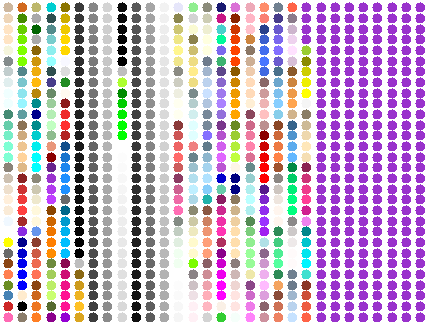
\includegraphics[width = 0.6\textwidth]{img/tk2dcolors.png}
  \caption{Mapping of the \texttt{group} argument to colors in the default tk2d window.}  
\end{figure}

If the data gets visualized with \texttt{ggobi}, the mapping from the \texttt{group} argument to the display items happens as shown in figure \ref{fig:ggobicolors}. Use the code

\begin{Schunk}
\begin{Sinput}
> nav <- navGraph(ng.test, settings = list(defaultDisplay = "ggobi"))
\end{Sinput}
\end{Schunk}
herefore.

\begin{figure}[h]
  \label{fig:ggobicolors}
  \centering
  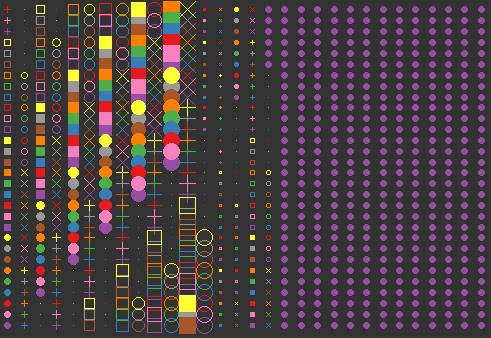
\includegraphics[width = 0.6\textwidth]{img/ggobicolors.png}
  \caption{Mapping of the \texttt{group} argument to colors in the ggobi dispaly.}  
\end{figure}

For the \modify{\texttt{tk2d}} display, the \texttt{group} variable could also be a vector of strings contained in the \texttt{colors()} output. For example

\begin{Schunk}
\begin{Sinput}
> x <- rep(1:3, each = 3)
> y <- rep(1:3, 3)
> ng.test <- ng_data(name = "test2", data = data.frame(x = x, y = y, 
+     z = 1:9), group = c("red", "red", "green", "blue", "blue", 
+     "blue", "blue", "orange", "orange"))
> nav <- navGraph(ng.test)
\end{Sinput}
\end{Schunk}

yield the output shown in figure \ref{fig:tk2dCols2}.

\begin{figure}[h]
  \label{fig:tk2dCols2}
  \centering
  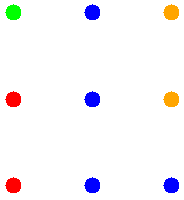
\includegraphics[width = 2cm]{img/tk2dcolors2.png}
  \caption{Mapping of the \texttt{group} argument containing color names.}  
\end{figure}


\section{Graph}
Defining an \texttt{NG\_graph} object happens in two stages. First, a \texttt{graph} object from the \texttt{graph} package has to be created. Second, a \texttt{NG\_graph} object gets created from the \texttt{graph} object. This has the advantage, that a \texttt{R} standard graph gets created using the full flexibility provided by other packages building on the \texttt{graph} package such as the \texttt{RGBL} and \texttt{Rgraphviz} package. 

\subsection{The \texttt{graph} package}
We recommend to take a brief look at the following vignettes in order to get an overview of some of the functionality of \texttt{R} handling graphs.

\begin{Schunk}
\begin{Sinput}
> vignette(package = "graph")
> vignette(package = "RBGL")
> vignette(package = "Rgraphviz")
\end{Sinput}
\end{Schunk}

The \texttt{graph()} package does, to our understanding, not deliver any simple creator functions, that is the user is left to use the \texttt{new()} creator function.

\begin{Schunk}
\begin{Sinput}
> adjM <- matrix(c(0, 4, 1, 0, 2, 0, 3, 2, 2, 2, 0, 0, 0, 2, 0, 
+     0), ncol = 4)
> rownames(adjM) <- c("A", "B", "C", "D")
> colnames(adjM) <- c("A", "B", "C", "D")
> G <- new("graphAM", adjMat = adjM, edgemode = "directed")
> G
\end{Sinput}
\begin{Soutput}
A graphAM graph with directed edges
Number of Nodes = 4 
Number of Edges = 8 
\end{Soutput}
\end{Schunk}
If the \texttt{Rgraphviz} package is installed, one can plot a \texttt{graph} object 
  \setkeys{Gin}{width=0.4\textwidth}
\begin{center}
\begin{Schunk}
\begin{Sinput}
> library(Rgraphviz)
> plot(G)
\end{Sinput}
\end{Schunk}
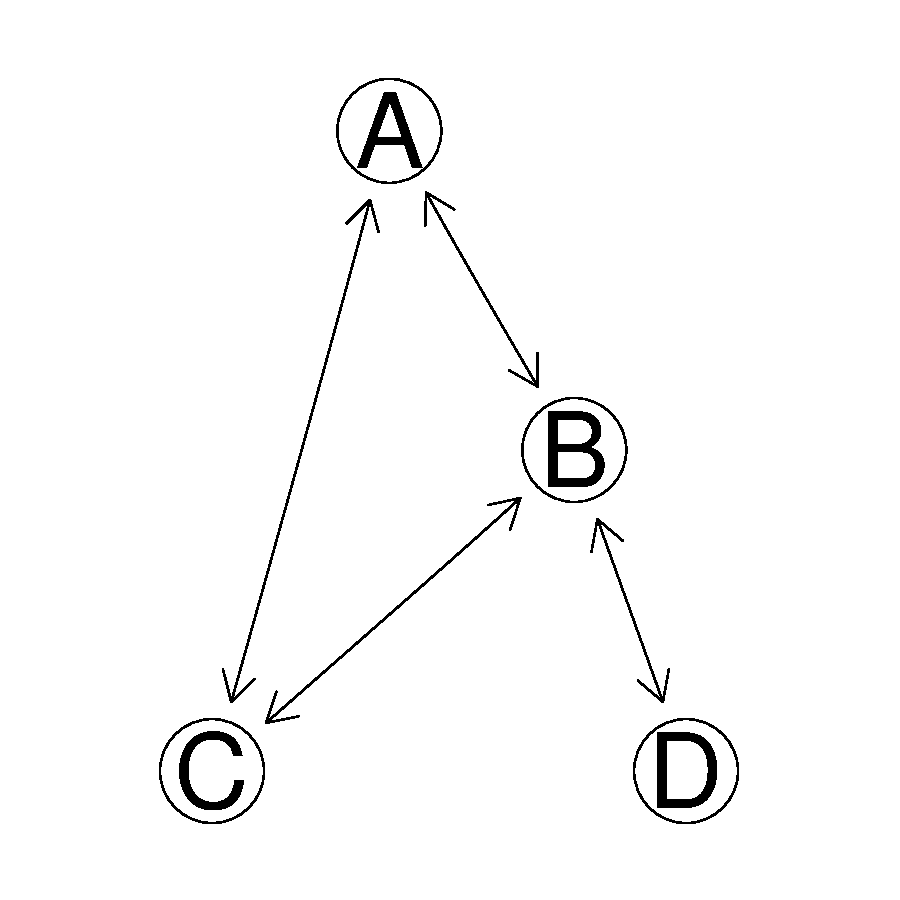
\includegraphics{sweave_p-031}
\end{center}

We have written some functions which ease the graph creation part. Often the users want to start from a complete variable graph. We provide the \texttt{completegraph} function which takes a vector of node names as the argument

\begin{center}
\begin{Schunk}
\begin{Sinput}
> V <- c("s.L", "s.W", "p.L", "p.W")
> G <- completegraph(V)
> plot(G, "neato")
\end{Sinput}
\end{Schunk}
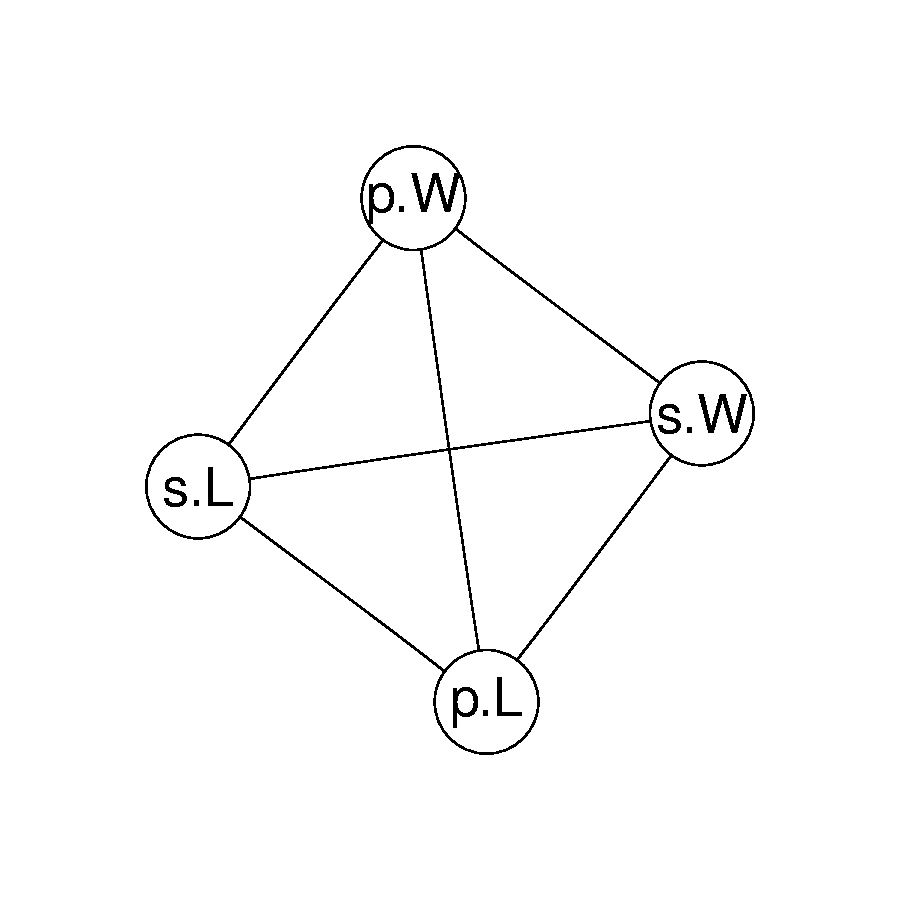
\includegraphics{sweave_p-032}
\end{center}

We also introduce the \texttt{newgraph} R function which either takes an adjacency- or a from-to-edge matrix to create a graph

\begin{center}
\begin{Schunk}
\begin{Sinput}
> from <- c("A", "A", "C", "C")
> to <- c("B", "C", "B", "D")
> ftEmat <- cbind(from, to)
> G <- newgraph(nodeNames = LETTERS[1:5], mat = ftEmat)
> plot(G, "neato")
\end{Sinput}
\end{Schunk}
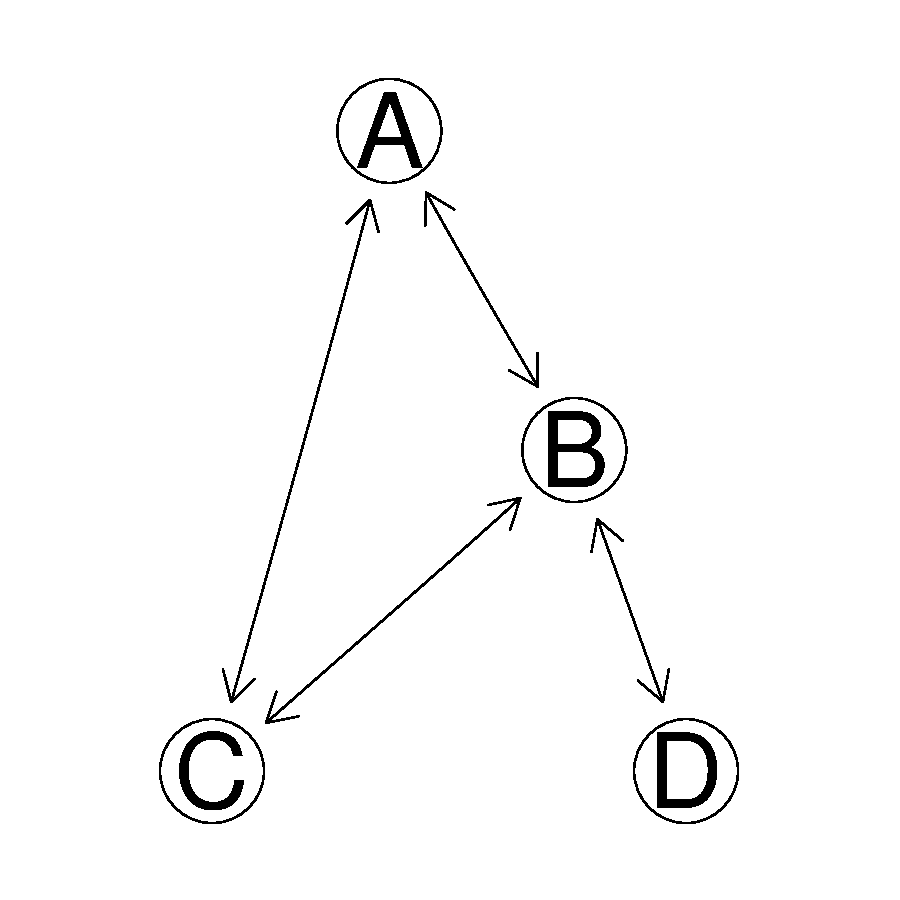
\includegraphics{sweave_p-033}
\end{center}
Note how the node ``E'' was added to the graph. Graphs can also be directed, however \texttt{RnavGraph} does not constrain the bullet in direction if an edge exists. Hence this feature is for the current \texttt{RnavGraph} version not from importance, however for completeness 

\begin{center}
\begin{Schunk}
\begin{Sinput}
> G <- newgraph(nodeNames = LETTERS[1:5], mat = ftEmat, directed = TRUE)
> plot(G, "neato")
\end{Sinput}
\end{Schunk}
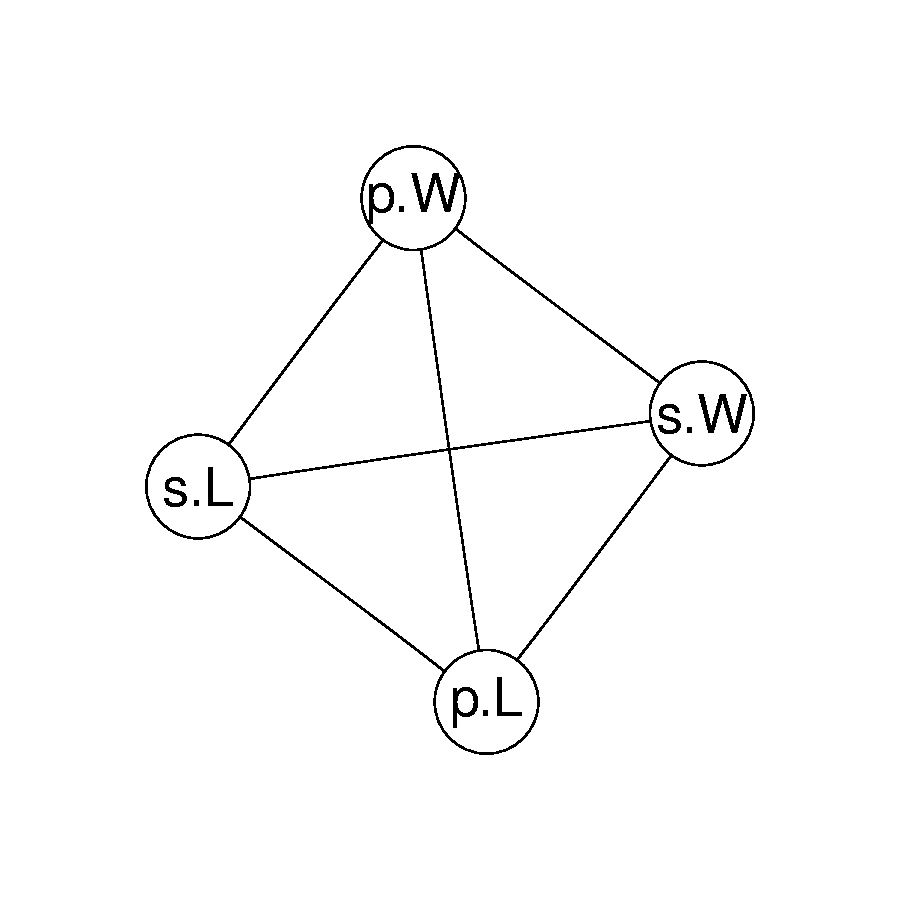
\includegraphics{sweave_p-034}
\end{center}

The from-to-edge matrix can also be numeric
\begin{center}
\begin{Schunk}
\begin{Sinput}
> from <- c(1, 1, 3, 3)
> to <- c(2, 3, 2, 4)
> ftEmat <- cbind(from, to)
> G <- newgraph(nodeNames = LETTERS[1:5], mat = ftEmat)
> plot(G, "neato")
\end{Sinput}
\end{Schunk}
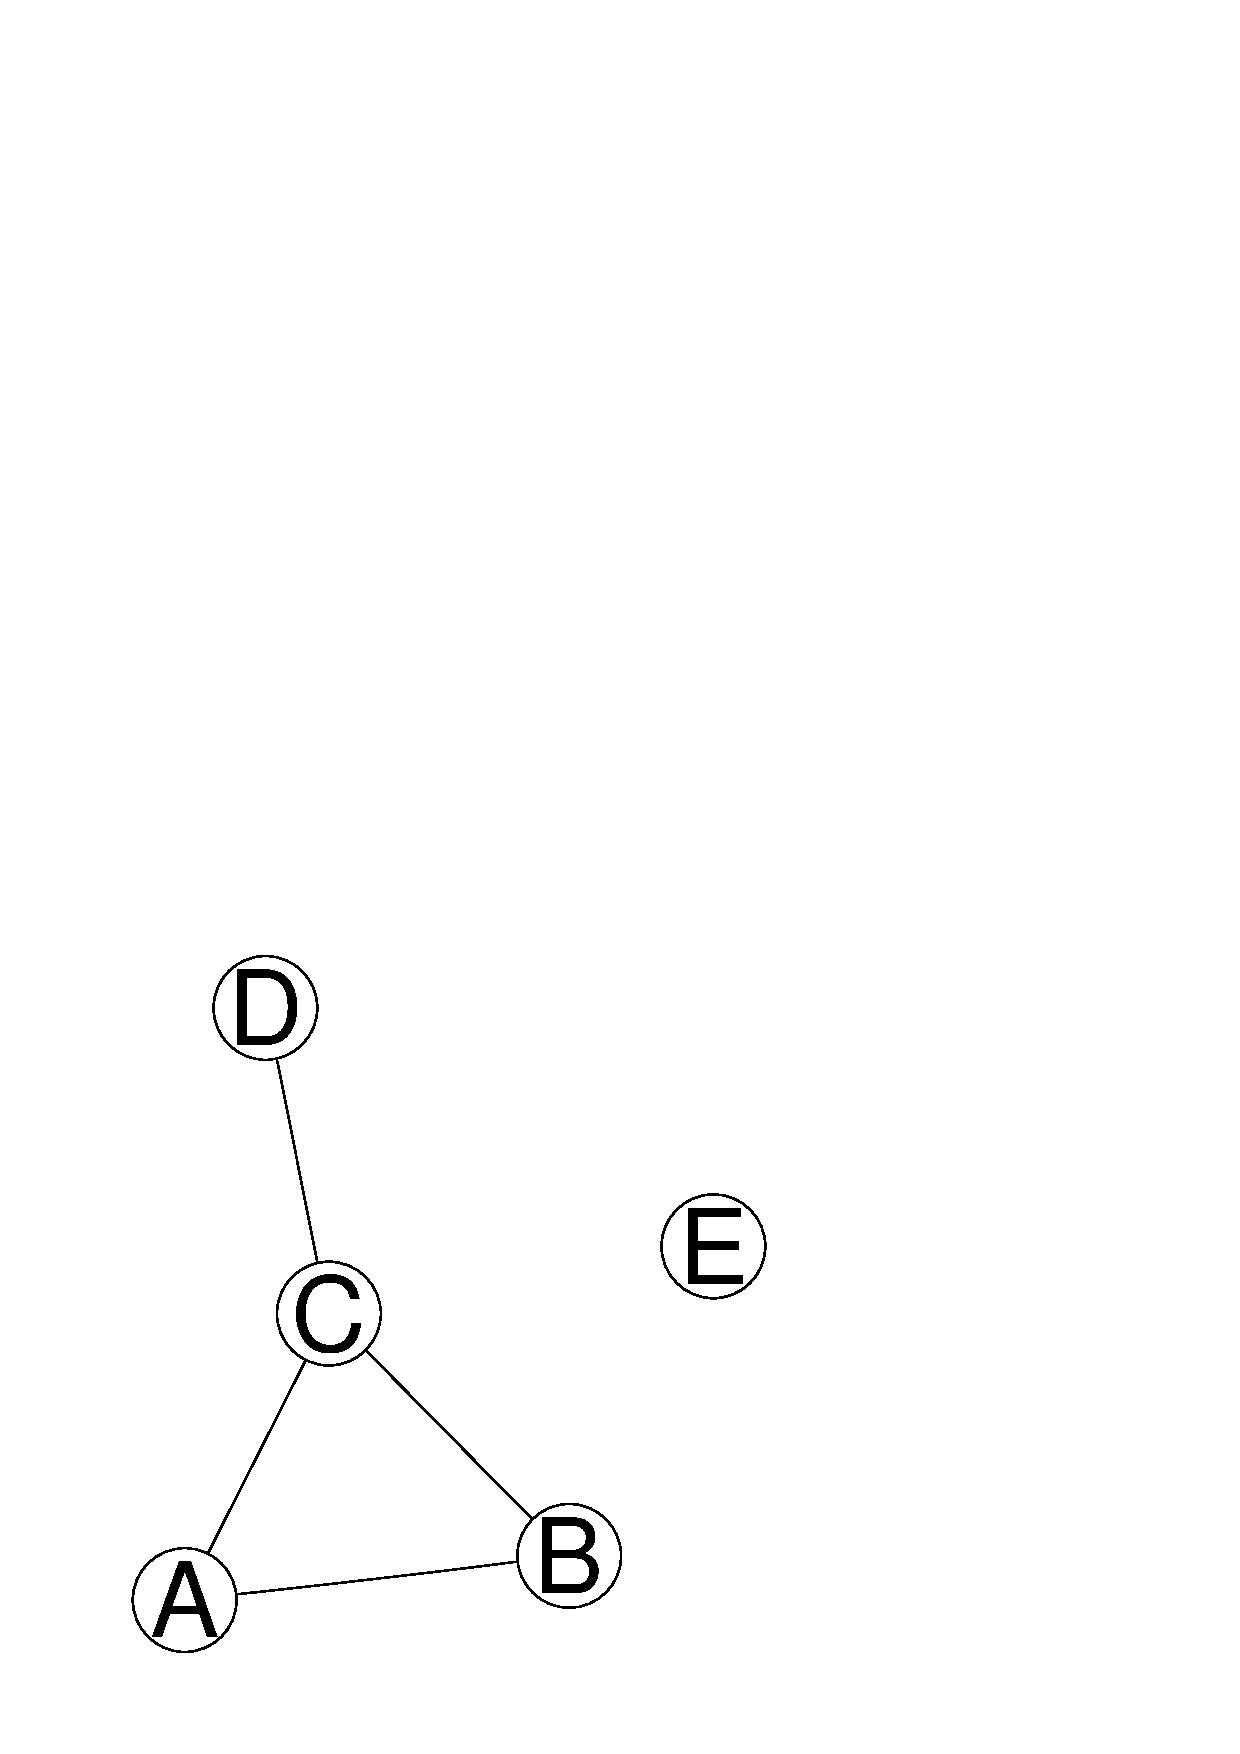
\includegraphics{sweave_p-035}
\end{center}

Weights can also added to Graphs via the weights argument. Note however that \texttt{navGraph} does not visualize them, however they might be important for greedy path finding algorithms
\begin{Schunk}
\begin{Sinput}
> weights <- c(2, 1, 3, 4)
> G <- newgraph(nodeNames = LETTERS[1:5], mat = ftEmat, weights = weights)
> edgeData(G, attr = "weight")
\end{Sinput}
\begin{Soutput}
$`A|B`
[1] 2

$`A|C`
[1] 1

$`B|A`
[1] 2

$`B|C`
[1] 3

$`C|B`
[1] 3

$`C|D`
[1] 4

$`C|A`
[1] 1

$`D|C`
[1] 4
\end{Soutput}
\end{Schunk}

Or alternatively you can add weights after the graph creation process
\begin{Schunk}
\begin{Sinput}
> G <- newgraph(nodeNames = LETTERS[1:5], mat = ftEmat, weights = weights, 
+     directed = TRUE)
> edgeData(G, attr = "weight")
\end{Sinput}
\begin{Soutput}
$`A|B`
[1] 2

$`A|C`
[1] 1

$`C|B`
[1] 3

$`C|D`
[1] 4
\end{Soutput}
\begin{Sinput}
> edgeData(G, from = "A", to = "B", attr = "weight")
\end{Sinput}
\begin{Soutput}
$`A|B`
[1] 2
\end{Soutput}
\begin{Sinput}
> edgeData(G, from = "A", to = "B", attr = "weight") <- 8
\end{Sinput}
\end{Schunk}

As mentioned earlier, the \texttt{newgraph} function takes also adjacency matrices as an argument, use the argument \texttt{isAdjacency=TRUE}
\begin{center}
\begin{Schunk}
\begin{Sinput}
> adjM <- matrix(c(0, 1, 1, 0, 1, 0, 1, 1, 1, 1, 0, 0, 0, 1, 0, 
+     0), ncol = 4)
> all(adjM == t(adjM))
\end{Sinput}
\begin{Soutput}
[1] TRUE
\end{Soutput}
\begin{Sinput}
> G <- newgraph(nodeNames = V, mat = adjM, isAdjacency = TRUE)
> plot(G, "neato")
\end{Sinput}
\end{Schunk}
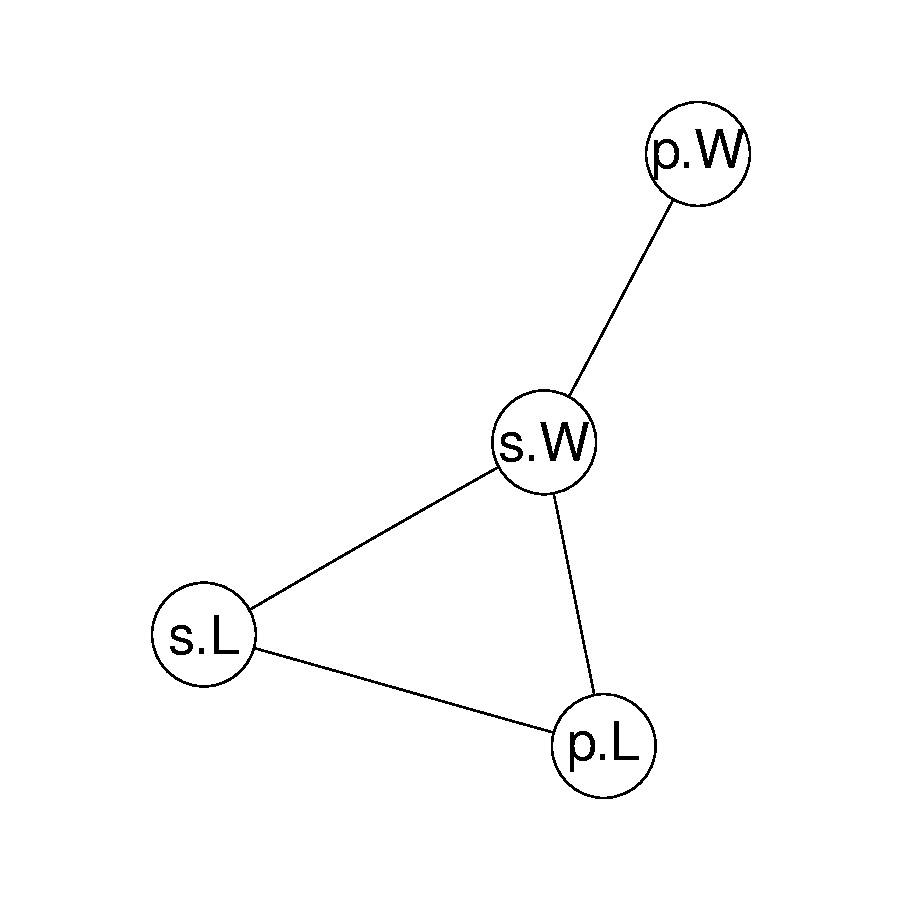
\includegraphics{sweave_p-038}
\end{center}
Note that all the graphs from the \texttt{graph} class have the function \texttt{nodes} and \texttt{edges} defined
\begin{Schunk}
\begin{Sinput}
> nodes(G)
\end{Sinput}
\begin{Soutput}
[1] "s.L" "s.W" "p.L" "p.W"
\end{Soutput}
\begin{Sinput}
> edges(G)
\end{Sinput}
\begin{Soutput}
$s.L
[1] "s.W" "p.L"

$s.W
[1] "s.L" "p.L" "p.W"

$p.L
[1] "s.L" "s.W"

$p.W
[1] "s.W"
\end{Soutput}
\end{Schunk}
If you use an adjacency matrix to create a graph, you can also pass on a weight matrix
\begin{Schunk}
\begin{Sinput}
> adjM <- matrix(c(0, 0, 1, 0, 1, 0, 1, 1, 0, 0, 0, 0, 0, 1, 0, 
+     0), ncol = 4)
> weightsM <- matrix(c(0, 0, 5, 0, 2, 0, 1, 3, 0, 0, 0, 0, 0, 7, 
+     0, 0), ncol = 4)
> G <- newgraph(nodeNames = V, mat = adjM, weights = weightsM, 
+     directed = TRUE, isAdjacency = TRUE)
> edgeData(G, attr = "weight")
\end{Sinput}
\begin{Soutput}
$`s.L|s.W`
[1] 2

$`s.W|p.W`
[1] 7

$`p.L|s.L`
[1] 5

$`p.L|s.W`
[1] 1

$`p.W|s.W`
[1] 3
\end{Soutput}
\end{Schunk}
Further the \texttt{ftM2adjM} function converts a from-to-edge matrix into a adjacency matrix
\begin{Schunk}
\begin{Sinput}
> ftM2adjM(ftEmat)
\end{Sinput}
\begin{Soutput}
  1 3 2 4
1 0 1 1 0
3 0 0 1 1
2 0 0 0 0
4 0 0 0 0
\end{Soutput}
\end{Schunk}

\subsubsection{linegraph and its complement}
After creating a variable graph, getting its linegraph and the complement of the linegraph yields the 3d- and 4d transition graph. We provide the \texttt{linegraph} and the \texttt{graph} package provides the \texttt{complement} function herefore. The linegraph has the separator \texttt{sep} argument to distinguish the node names. You must chose a string that does not occur within the node names.

\begin{Schunk}
\begin{Sinput}
> G <- completegraph(V)
> LG <- linegraph(G, sep = "::")
> nodes(LG)
\end{Sinput}
\begin{Soutput}
[1] "s.L::s.W" "s.L::p.L" "s.L::p.W" "s.W::p.L" "s.W::p.W" "p.L::p.W"
\end{Soutput}
\end{Schunk}
\modify{Notice, if G had edge weights, then they are lost now. Also the line graph is only defined for undirected graphs at the moment.}




\subsection{The \texttt{NG\_data} object}
The user can get his graphs in whatever ways he want. In the end, the node names must be in sync with the shortnames or names of the \texttt{NG\_data} object, and the graph must be from the \texttt{graph} class and subsequently the \texttt{NG\_graph} class.\\

It stays to create an \texttt{NG\_data} object

\begin{Schunk}
\begin{Sinput}
> ng.LG <- ng_graph(name = "3D Transition", graph = LG, sep = "++", 
+     layout = "circle")
\end{Sinput}
\begin{Soutput}
[ng_graph]: warning, sep does not occur in some node names
\end{Soutput}
\begin{Sinput}
> ng.LG
\end{Sinput}
\begin{Soutput}
NG_graph object from ng_graph()
name: 3D Transition 
layout: circle 
\end{Soutput}
\end{Schunk}
Note that you have to specify the \texttt{sep} argument again. The reason herefore is that you could pass on any graph with any dimensionality of node names (e.g. ``A:B:C:D'' for four dimensions). In addition, you can specify the graph layout. Currently \texttt{circle}, \texttt{random} \modify{(currently not working)}, \texttt{kamadaKawaiSpring} and \texttt{fruchtermanReingold} are possible options for the layout. We use the \texttt{RBGL} package to get the latter two layouts. The complement does not need any special considerations
\begin{Schunk}
\begin{Sinput}
> LGnot <- complement(LG)
> ng.LGnot <- ng_graph(name = "4D Transition", graph = LGnot, sep = "::", 
+     layout = "circle")
\end{Sinput}
\end{Schunk}
The name of each \texttt{NG\_graph} object, as for the \texttt{NG\_data} object, must be unique within all graphs passed on to the \texttt{navGraph} function. \texttt{NG\_graph} objects can be plotted
  \setkeys{Gin}{width=0.8\textwidth}
\begin{center}
\begin{Schunk}
\begin{Sinput}
> par(mfrow = c(1, 2))
> plot(ng.LG)
> plot(ng.LGnot)
\end{Sinput}
\end{Schunk}
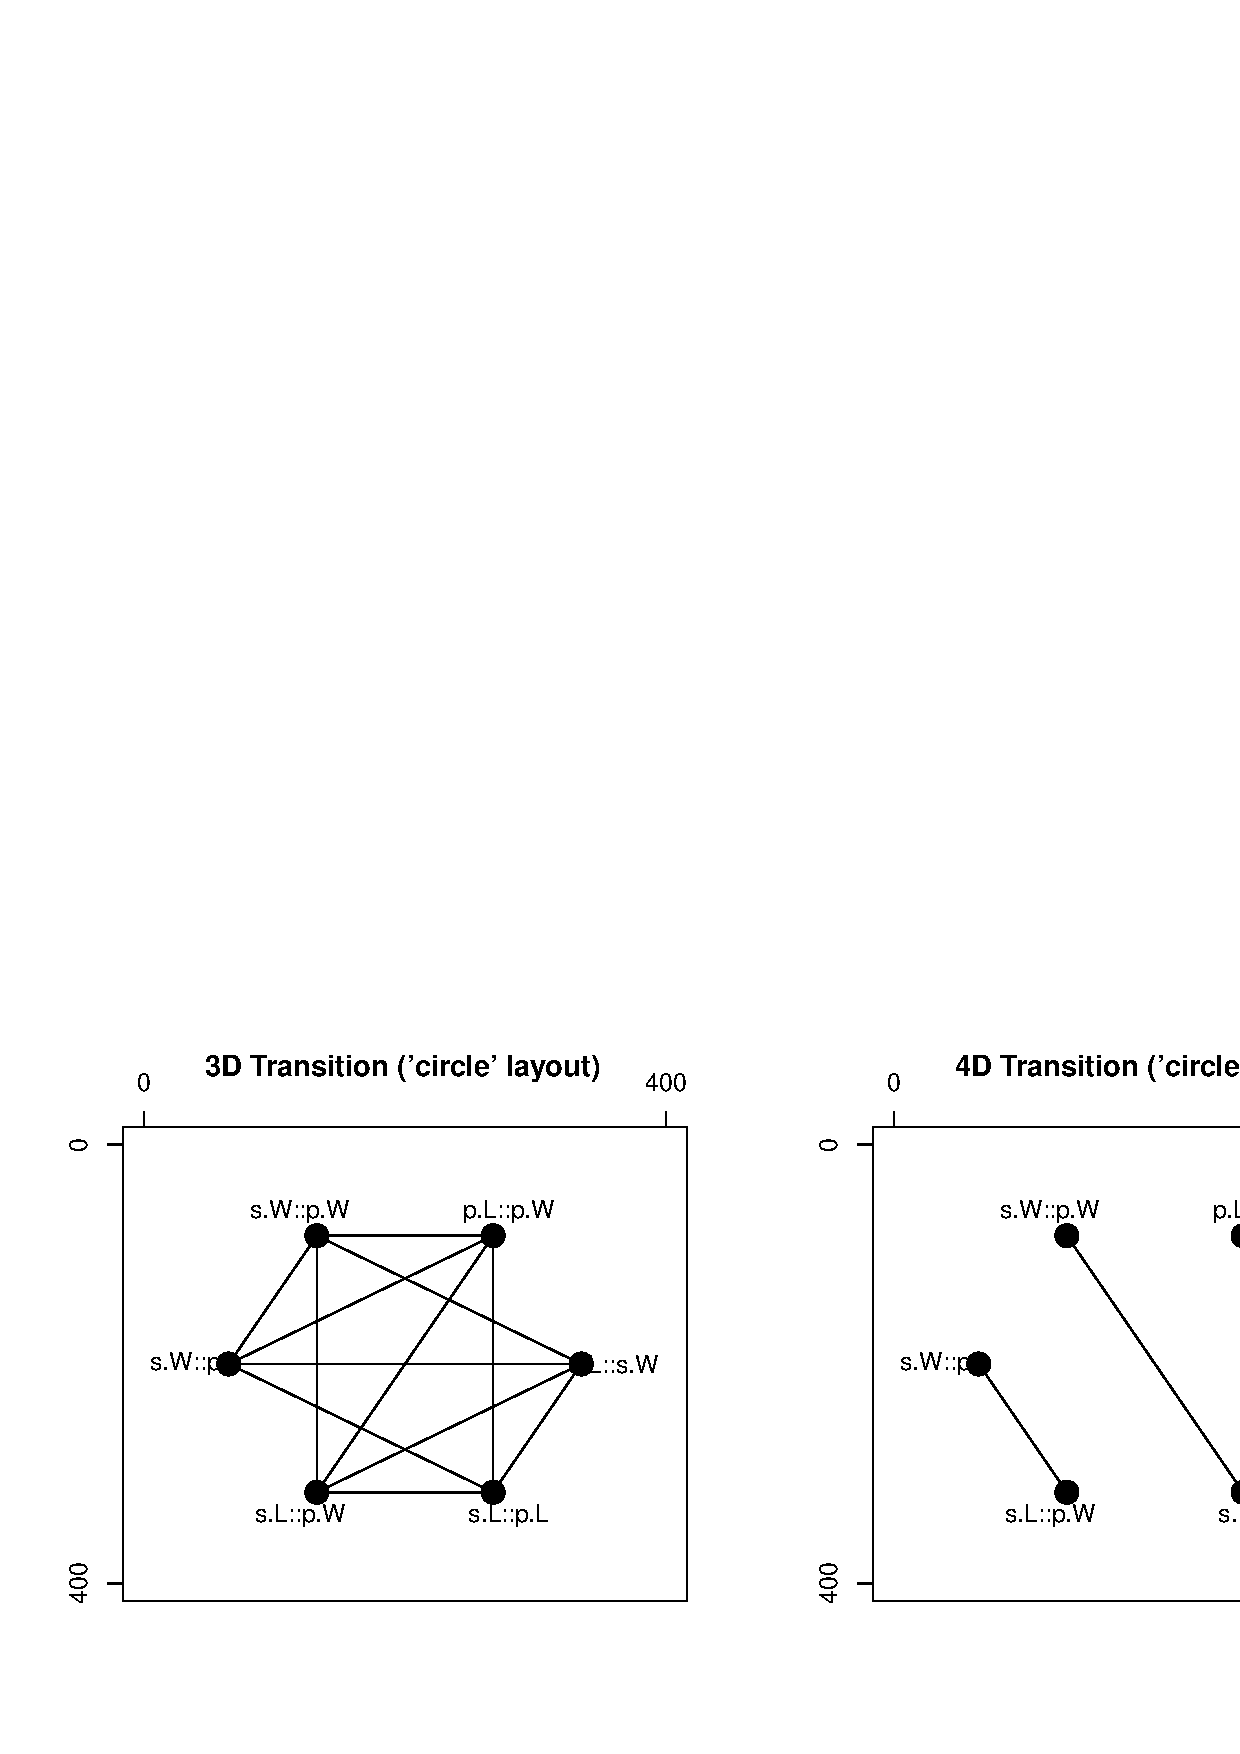
\includegraphics{sweave_p-045}
\end{center}

As for the \texttt{NG\_data} object, you can access or modify with the \texttt{ng\_get} and \texttt{ng\_set} function, respectively.
\begin{Schunk}
\begin{Sinput}
> ng_get(ng.LG)
\end{Sinput}
\begin{Soutput}
Get what? Possible options are: name, graph, visitedEdges, layout
\end{Soutput}
\begin{Sinput}
> ng_set(ng.LG, "name") <- "3d transition graph"
\end{Sinput}
\end{Schunk}
\modify{Careful, some things are linked: graph, visitedEdges and layout. Changing one should affect the whole object (which it does not at the moment)}.

\section{Visualization Instructions}
Once the \texttt{NG\_data} and \texttt{NG\_graph} objects have been defined, they have to be connected with some visualization instructions. That is, the visualization instructions tell \texttt{navGraph} what and how \texttt{navGraph} should visualize when the ball gets moved along the edges of the graph. Conceptually, \texttt{navGraph} allows for any visualization of the data, as long the user can implement them. That is, there are no constrains to dimensionality of data represented by a node or the ``morphing'' defined along an edge. \modify{This feature is not documented yet, however you can achieve this with the \texttt{ng\_2d\_myplot} function}. However the \texttt{RnavGraph} package implements the 2d-scatterplot example \modify{for the moment} and provides an interface for the user to implement their own --possibly new-- ideas.\\

For the 2d- scatterplot example, we need a device that plots some objects at the $x$ and $y$ euclidean coordinate. The objects could be either dots, images, glyphs, text or anything else you can imagine (and implement). There are many plotting devices available in \texttt{R} (e.g. traditional graphics, grid, rgl and ggobi) and \texttt{navGraph} can deal with most of them. However when it comes to speed and \modify{double buffering}, only few of them produce satisfactory output. In addition, different devices allow for different objects to be plotted. \modify{We have implemented a new device, lets call it \texttt{tk2d},} that builds upon the tk canvas widget (so does the interactive graph). Alternatively to \texttt{tk2d} one can use the \texttt{rggobi} package and \texttt{ggobi} to visualize the scatterplots. \texttt{ggobi} however does only allow to visualize dots, rectangles and \modify{crosses} in different colors. \texttt{Ggobi} has not been maintained for a while and hence does not run well on \modify{all to my knowledge?} current operating systems. For what follows, we will give a detailed explanation of each device. \modify{Most likely you only want to read the \texttt{tk2d} and \texttt{ggobi} subsection and then return to this section once you have more custom needs}. 


\subsection{\texttt{tk2d}}
The \texttt{tk2d} device can either display dots, images, glyphs or text (strings). 

\begin{figure}[h]
\begin{center}
\begin{tikzpicture}
  [dot/.style={circle, draw=black!50, fill=black!50, minimum size=1.5mm}]
  

    %% 2d Scatterplot  dots
  \begin{scope}
    \node at ( -0.8, -0.8) [dot] {};
    \node at ( -0.2, -0.6) [dot] {};
    \node at ( 2.6, 0.6) [dot] {};
    \node at ( 3, -0.4) [dot] {};
    \node at ( 1.6, 0.8) [dot] {};
    \node at ( 1.0, 1) [dot] {};
    \node at ( -1, 0.6) [dot] {};
    \node at ( 0, 0.6) [dot] {};
    \node at ( 1.2, -0.6) [dot] {};
    \node at ( 2, -1) [dot] {};
    \draw (-1.6,-1.6) -- (3.6,-1.6) -- (3.6,1.6) -- (-1.6,1.6) -- (-1.6,-1.6);
    \node at (-1.6,1.8) [anchor=west] {linked 2d dots scatterplot};
  \end{scope}

  
  
  
  %% 2d Scatterplot  images
  \begin{scope}[shift = {(8.4,0)}]
    \node at ( -0.8, -0.8) {\pgfbox[center,center]{\pgfuseimage{f1_1}}};
    \node at ( -0.2, -0.6) {\pgfbox[center,center]{\pgfuseimage{f1_2}}};
    \node at ( 2.6, 0.6) {\pgfbox[center,center]{\pgfuseimage{f2_1}}};
    \node at ( 3, -0.4) {\pgfbox[center,center]{\pgfuseimage{f2_2}}};
    \node at ( 1.6, 0.8) {\pgfbox[center,center]{\pgfuseimage{m1_1}}};
    \node at ( 1.0, 1) {\pgfbox[center,center]{\pgfuseimage{m1_2}}};
    \node at ( -1, 0.6) {\pgfbox[center,center]{\pgfuseimage{m2_1}}};
    \node at ( 0, 0.6) {\pgfbox[center,center]{\pgfuseimage{m3_1}}};
    \node at ( 1.2, -0.6) {\pgfbox[center,center]{\pgfuseimage{m4_1}}};
    \node at ( 2, -1) {\pgfbox[center,center]{\pgfuseimage{m4_2}}};
    \draw (-1.6,-1.6) -- (3.6,-1.6) -- (3.6,1.6) -- (-1.6,1.6) -- (-1.6,-1.6);
    \node at (-1.6,1.8) [anchor=west] {linked 2d image scatterplot};
  \end{scope}



  \begin{scope}[shift={(0,-5)}]
    \newcommand{\radius}{0.4}

    \foreach \x/\y/\a/\b/\c/\d in {
      -0.8/-0.8/  0.8/0.5/0.6/0.2,    % f1_1
      -0.2/-0.6/  0.8/0.4/0.7/0.2,    % f1_2
       2.6/0.6/   0.2/0.9/0.4/0.7,    % f2_1
      3/-0.4/     0.1/0.9/0.5/0.5,    % f2_2
      1.6/0.8/    0.3/0.7/0.4/0.6,    % m1_1
      1.0/1/      0.25/0.6/0.5/0.5,    % m1_2
      -1/0.6/     0.1/0.9/0.5/0.5,    % m2_1
      0/0.6/      0.4/0.8/0.4/0.2,    % m3_1
      1.2/-0.6/   0.6/0.6/0.1/0.8,    % m4_1
      2/-1/       0.6/0.6/0.1/0.8     % m4_2
    } {
      \foreach \alpha/\perc in {0/\a,40/\b,80/\c,120/\d,160/\a,200/\c,240/\d,280/\b,320/\d} {
        \coordinate (\alpha) at ($(\x,\y)!\perc!\alpha:(\x,\y+\radius)$) {};
      }
      \draw[fill = black!20] (0) -- (40) -- (80) -- (120) -- (160)
      -- (200) -- (240) -- (280) -- (320) -- cycle;
    }
    \draw (-1.6,-1.6) -- (3.6,-1.6) -- (3.6,1.6) -- (-1.6,1.6) -- (-1.6,-1.6);
    \node at (-1.6,1.8) [anchor=west] {linked 2d glyph scatterplot};
  \end{scope}

    %% 2d Scatterplot  text
  \begin{scope}[shift = {(8.4,-5)}]
    \node at ( -0.8, -0.8) {Jane};
    \node at ( -0.2, -0.6) {Jane};
    \node at ( 2.6, 0.6) {Lea};
    \node at ( 3, -0.4) {Lea};
    \node at ( 1.6, 0.8) {Max};
    \node at ( 1.0, 1) {Max};
    \node at ( -1, 0.6) {Joe};
    \node at ( 0, 0.6) {Mike};
    \node at ( 1.2, -0.6) {Bill};
    \node at ( 2, -1) {Bill};
    \draw (-1.6,-1.6) -- (3.6,-1.6) -- (3.6,1.6) -- (-1.6,1.6) -- (-1.6,-1.6);
    \node at (-1.6,1.8) [anchor=west] {linked 2d text scatterplot};
  \end{scope}


\end{tikzpicture}
\end{center}
  \caption{\texttt{tk2d} can visualize dots, images, glyphs and text.}
  \label{fig:tk2d}
\end{figure}

Once the \texttt{tk2d} device is started, there is a whole set of interaction tools like brushing, changing colors, resizing images etc. We will discuss them in the ``Starting a \texttt{navGraph} Session'' section. For now lets define some visualization instructions that use the \texttt{tk2d} device and only show dots

\begin{Schunk}
\begin{Sinput}
> viz1 <- ng_2d(data = ng.iris, graph = ng.lg)
> viz1
\end{Sinput}
\begin{Soutput}
tk2d scatter plot: ng_2d()
Graph: 3D Transition 
Data: iris 
\end{Soutput}
\end{Schunk}
Notice the output of the \texttt{viz1} object. It says that it addresses the \texttt{tk2d} device which displays a scatterplot and that it connects the \texttt{NG\_graph} object with the name ``3D Transition'' with the \texttt{NG\_data} object with the name ``iris''. Hence if you weren't to choose the graph and data names unique, \texttt{navGraph} would not know how to link them correctly. \texttt{navGraph} has no bound on the number of visualization instructions you can pass on as an argument. So lets define another \texttt{tk2d} visualization object
\begin{Schunk}
\begin{Sinput}
> viz2 <- ng_2d(data = ng.iris, graph = ng.lgnot)
\end{Sinput}
\end{Schunk}

\subsubsection{Working with Images (from some text source)}
The main reason we implemented the \texttt{tk2d} device is because we wanted the \texttt{RnavGraph} package to be useful to explore image data. All images get imported as tcl \texttt{image} objects since they later will be displayed on a tk canvas widget. This has the implication that the user needs a running \texttt{Img} tcl extension set up for the tcltk version R connects to via the \texttt{tcltk} R package. If the images however eventually exist as an R object of some sort (e.g. a matrix), the tcl \texttt{Img} extension is not needed. For the examples in this vignette and for some of the demos, we require the \texttt{RnavGraphImageData} package. 
\begin{Schunk}
\begin{Sinput}
> library(RnavGraphImageData)
\end{Sinput}
\end{Schunk}
you can get an overview of the data provided by the package with
\begin{Schunk}
\begin{Sinput}
> data(package = "RnavGraphImageData")
\end{Sinput}
\end{Schunk}
\modify{Much of this data is from the webpage of Sam Roweis \tiny{http://www.cs.nyu.edu/$\sim$roweis/data.html}}.\\

Lets start with the USPS \texttt{digits} image data
\begin{Schunk}
\begin{Sinput}
> data(digits)
> dim(digits)
\end{Sinput}
\begin{Soutput}
[1]   256 11000
\end{Soutput}
\end{Schunk}
from the help documentation (\modify{not done yet}) for the data set
\begin{Schunk}
\begin{Sinput}
> help("digits")
\end{Sinput}
\end{Schunk}
we get that the \texttt{digits} data consists of \modify{$16\times 16$ 8-bit grayscale images of ``0'' through ``9''; 1100 examples of each class}. That is, one image is stored in one column (which is often the case in the machine learning field). For example the data of one handwritten $8$ is 
\begin{Schunk}
\begin{Sinput}
> matrix(digits[, 7 * 1100 + 1], ncol = 16, byrow = FALSE)
\end{Sinput}
\end{Schunk}
\begin{tiny}
\begin{Schunk}
\begin{Soutput}
      [,1] [,2] [,3] [,4] [,5] [,6] [,7] [,8] [,9] [,10] [,11] [,12] [,13] [,14] [,15] [,16]
 [1,]    0    0    0    7   71  156  156  156  156   125    37     0     0     0     0     0
 [2,]    0   19  170  217  255  255  255  252  252   255   173     8     0     0     0     0
 [3,]    8  255  255  247  186  120   87   66   66    87   144   161     0     0     0     0
 [4,]    7  244  255  127    0    0    0    0    0     0    44    34     0     0    24    13
 [5,]    0  100  255  246  166   27    0    0    0     0     0     0    32   173   214    88
 [6,]    0    1   85  240  255  224   41    0    0    30   119   174   138   121    15     0
 [7,]    0    0    0   61  255  255  190   94  121   242   255   220    91     5     0     0
 [8,]    0    0    0    1  117  255  255  255  255   185   105    18     0     0     0     0
 [9,]    0    0    1   79  237  250  253  255  228    32     0     0     0     0     0     0
[10,]    0   34  129  255  200   31   86  238  255   131     0     0     0     0     0     0
[11,]    4  193  253  163   13    0    0  129  255   213    21     0     0     0     0     0
[12,]   93  255  195    0    0    0    0   20  213   255    81     0     0     0     0     0
[13,]  131  255  123    0    0    0    0    8  202   255   153     0     0     0     0     0
[14,]   89  255  249  188  124   88   88  178  255   228    30     0     0     0     0     0
[15,]    0   17  172  255  255  255  255  255  243    49     0     0     0     0     0     0
[16,]    0    0    5   67  154  154  154  130   40     0     0     0     0     0     0     0
\end{Soutput}
\end{Schunk}
\end{tiny}
Hence the gray scales are coded from $0$ to $255$. Since visualizing $11000$ digits is computationally expensive, we will continue with a sub-sample of the data
\begin{Schunk}
\begin{Sinput}
> sel <- sample(x = 1:11000, size = 600)
> p.digits <- digits[, sel]
\end{Sinput}
\end{Schunk}
% $
In order for \texttt{tk2d} to be able to display the images, they need to be wrapped into a \texttt{NG\_image} object. Now, contrary to all the \texttt{NG\_...} objects we have encountered so far, the \texttt{NG\_image} class does not wrap the image data within itself. The \texttt{NG\_image} object contains only the names (character strings) of the images that (the names) tcl did automatically assign. That is, when importing an image into tcl, tcl names them consecutively, i.e. \texttt{image1}, \texttt{image2}, ..., so that they can readily be displayed when needed. Coming back to our \texttt{digits} example, the \texttt{ng\_image\_array\_gray} R function creates a \texttt{NG\_image} object from a \texttt{data.frame} object with values ranging from $0$ to $255$.
\begin{Schunk}
\begin{Sinput}
> ng.i.digits <- ng_image_array_gray("USPS Handwritten Digits", 
+     p.digits, 16, 16, invert = TRUE, img_in_row = FALSE)
\end{Sinput}
\end{Schunk}

the images can be seen with
\begin{Schunk}
\begin{Sinput}
> ng.i.digits
\end{Sinput}
\end{Schunk}
which would yield something like (it's random because of the sampling!)
\begin{center}
  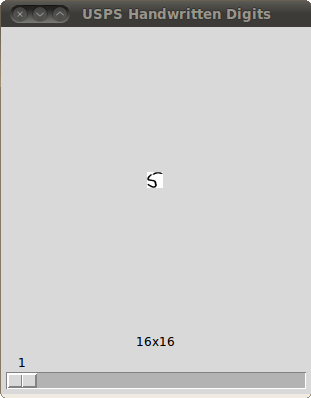
\includegraphics[width = 5cm]{img/tk2dimages1.png}
\end{center}
where the scroll bar can be used to navigate through all the images. The name you specified does not have to be unique since here the image ids are the only important part. \modify{The name is only used for the \texttt{print} output of the \texttt{NG\_image} object}. We also need data on the images. Many scenario are possible, i.e. we could have measured data for each image or we could perform some kind of feature extraction for each image or we reduce the dimensionality (number of pixel) of each image to something manageable, say $4$ or $5$ dimension --rather than the commonly conveniently chosen two dimensions--. For the rest of this vignette, we choose the dimensionality reduction approach using isomap provided in the \texttt{vegan} (or also by the \texttt{RDRToolbox}) R package. 
\begin{Schunk}
\begin{Sinput}
> library(vegan)
\end{Sinput}
\end{Schunk}
We need to transpose the \texttt{digit} data first, since each image is saved as one column and not within a row (the statistics- and computer science field seem to disagree on a common convention).
\begin{Schunk}
\begin{Sinput}
> p.digitsT <- t(p.digits)
\end{Sinput}
\end{Schunk}
Next, we need to generate a distance matrix (euclidean distance of one image to another) and perform isomap on the distances
\begin{Schunk}
\begin{Sinput}
> dise <- vegdist(p.digitsT, method = "euclidean")
> ord <- isomap(dise, k = 8, ndim = 6, fragmentedOK = TRUE)
\end{Sinput}
\end{Schunk}
Next we create an \texttt{NG\_data} object
\begin{Schunk}
\begin{Sinput}
> digits_group <- rep(c(1:9, 0), each = 1100)
> ng.iso.digits <- ng_data(name = "ISO_digits", data = data.frame(ord$points), 
+     shortnames = paste("i", 1:6, sep = ""), group = digits_group[sel], 
+     labels = as.character(digits_group[sel]))
\end{Sinput}
\end{Schunk}
and the \texttt{NG\_graph} objects
\begin{Schunk}
\begin{Sinput}
> V <- shortnames(ng.iso.digits)
> G <- completegraph(V)
> LG <- linegraph(G)
> LGnot <- complement(LG)
> ng.LG <- ng_graph(name = "3D Transition", graph = LG)
> ng.LGnot <- ng_graph(name = "4D Transition", graph = LGnot)
\end{Sinput}
\end{Schunk}
%$
And finally, the visualization instruction allow for adding the images to the \texttt{tk2d} plot
\begin{Schunk}
\begin{Sinput}
> vizDigits1 <- ng_2d(data = ng.iso.digits, graph = ng.LG, images = ng.i.digits)
> vizDigits2 <- ng_2d(data = ng.iso.digits, graph = ng.LGnot, images = ng.i.digits)
\end{Sinput}
\end{Schunk}
Starting a \texttt{navGraph} session is simple (but in more detail discussed later on)
\begin{Schunk}
\begin{Sinput}
> nav <- navGraph(data = ng.iso.digits, graph = list(ng.LG, ng.LGnot), 
+     viz = list(vizDigits1, vizDigits2))
\end{Sinput}
\end{Schunk}


\begin{center}
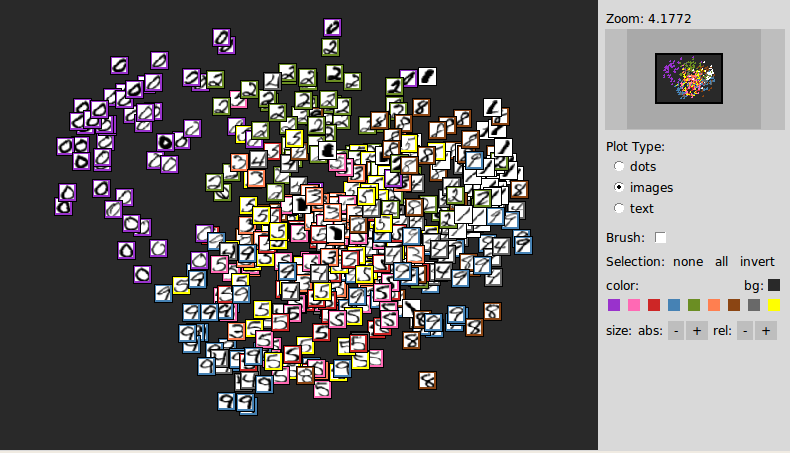
\includegraphics[width = 0.6 \textwidth]{img/imageDigits.png}  
\end{center}

For other examples of importing greyscale images from txt data file see the \texttt{ng\_2d\_images\_alpha\_letter}, \texttt{ng\_2d\_images\_alpha\_letter} and \texttt{ng\_2d\_images\_umist\_faces} demos.


\subsubsection{Working with color Images (jpeg, png, etc...)}

If your image data source is a bmp, gif, ico, jpeg, pcx, pixmap, png, ppm, postscript, sgi, sun, tga, tiff, window, xbm or xpm file, the \texttt{ng\_image\_files} R function helps you to import the images into the \texttt{tcl} layer provided the \texttt{Img} tcl extension works properly. If you need to precess the image data in \texttt{R}, the R packages \ref{tab:ImagesInR} provide some functionality, however not for all the formats the \texttt{Img} tcl extension is capable of importing. Note however with the \texttt{shell} R command and an installed Imagemagik you can convert any images to almost any format you could wish for.\\
\begin{Schunk}
\begin{Sinput}
> shell("convert image.png image.jpg")
\end{Sinput}
\end{Schunk}

\begin{table}[h]
  \label{tab:ImagesInR}
  \centering
  \begin{tabular}{llll}
    \hline
    Function & Package & Image Format & Returned Object\\
    \hline
    \texttt{read.pnm} & \texttt{pixmap} & pbm, pgm, ppm & objects of diverse pixmap classes\\
    \texttt{read.jpeg} & \texttt{rimage} & jpeg & image.matrix object\\
    \texttt{readRiff} & \texttt{rtiff} & tiff & pixmap objcet\\
    \texttt{readPNG} & \texttt{png} & png & array\\
    \hline
  \end{tabular}    
  \caption{\modify{Table (almost) directly from the useR book "Morphometrics with R" page 33.}}
\end{table}


We work with a data set from the Library of Amsterdam \modify{http://staff.science.uva.nl/$\sim$aloi/}. The download is the ``Quater resolution (192 $\times$ 144)'' which whose size is 60MB and contains $1000-250$ objects with each three different viewing angles \modify{2250} images. We have attached a resized version ($38x29$ pixels) in the \texttt{RnavGraphImageData} package in order to save space. 

\begin{center}
  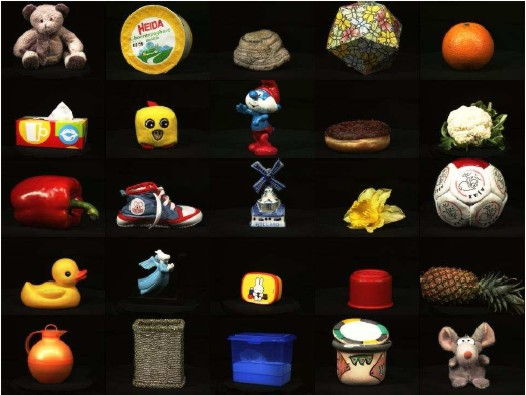
\includegraphics[width = 0.6\textwidth]{img/aloi.jpg}
\end{center}

The path to the images is
\begin{Schunk}
\begin{Sinput}
> imgPath <- system.file("aloi_small", package = "RnavGraphImageData")
> aloi_images <- list.files(path = imgPath, full.names = TRUE)
> length(aloi_images)
\end{Sinput}
\begin{Soutput}
[1] 2250
\end{Soutput}
\begin{Sinput}
> aloi_images[1:5]
\end{Sinput}
\begin{Soutput}
[1] "/usr/local/lib/R/site-library/RnavGraphImageData/aloi_small/1000_c.png"
[2] "/usr/local/lib/R/site-library/RnavGraphImageData/aloi_small/1000_l.png"
[3] "/usr/local/lib/R/site-library/RnavGraphImageData/aloi_small/1000_r.png"
[4] "/usr/local/lib/R/site-library/RnavGraphImageData/aloi_small/251_c.png" 
[5] "/usr/local/lib/R/site-library/RnavGraphImageData/aloi_small/251_l.png" 
\end{Soutput}
\end{Schunk}
We sample 400 images, so that we do not have to deal with all 2250 images.
\begin{Schunk}
\begin{Sinput}
> sel <- sample(1:length(aloi_images), replace = FALSE)
> p.aloi_images <- aloi_images[sel]
\end{Sinput}
\end{Schunk}


\modify{Note that the \texttt{rimage} package needs the \texttt{fftw-dev} (in ubuntu) package to perform Fast Fourier Transformations.}\\


Now, lets import the images first into the tcl layer, herefore the \modify{universal function (for jpg,png, ...)} is \texttt{ng\_image\_files}:
\begin{Schunk}
\begin{Sinput}
> ng.i.objects <- ng_image_files(name = "ALOI objects", path = p.aloi_images)
\end{Sinput}
\end{Schunk}
and again, you can see the images using
\begin{Schunk}
\begin{Sinput}
> ng.i.objects
\end{Sinput}
\end{Schunk}

In order to work with the image date we use the \texttt{readPNG} function from the \texttt{png} package. \modify{\texttt{readPNG} returns a three dimensional array with the red-blue-green contents for each pixel. For the ease of our demonstration we just get for each image the sum of each, red,green,blue, content}
\begin{Schunk}
\begin{Sinput}
> library(png)
> imgData <- t(sapply(p.aloi_images, FUN = function(path) {
+     x <- readPNG(path)
+     r <- sum(x[, , 1])
+     g <- sum(x[, , 2])
+     b <- sum(x[, , 3])
+     return(c(r, g, b))
+ }))
\end{Sinput}
\end{Schunk}
Initializing a \texttt{navGraph} session on this data with the images stays the same as in the previous example
\begin{Schunk}
\begin{Sinput}
> ng.iso.objects <- ng_data(name = "ISO_objects", data = data.frame(imgData), 
+     shortnames = paste("i", 1:3, sep = ""))
> V <- shortnames(ng.iso.objects)
> G <- completegraph(V)
> LG <- linegraph(G)
> LGnot <- complement(LG)
> ng.LG <- ng_graph(name = "3D Transition", graph = LG)
> ng.LGnot <- ng_graph(name = "4D Transition", graph = LGnot)
> vizObjects1 <- ng_2d(data = ng.iso.objects, graph = ng.LG, images = ng.i.objects)
> vizObjects2 <- ng_2d(data = ng.iso.objects, graph = ng.LGnot, 
+     images = ng.i.objects)
> nav <- navGraph(data = ng.iso.objects, graph = list(ng.LG, ng.LGnot), 
+     viz = list(vizObjects1, vizObjects2))
\end{Sinput}
\end{Schunk}

and you should expect to see something like

\begin{center}
  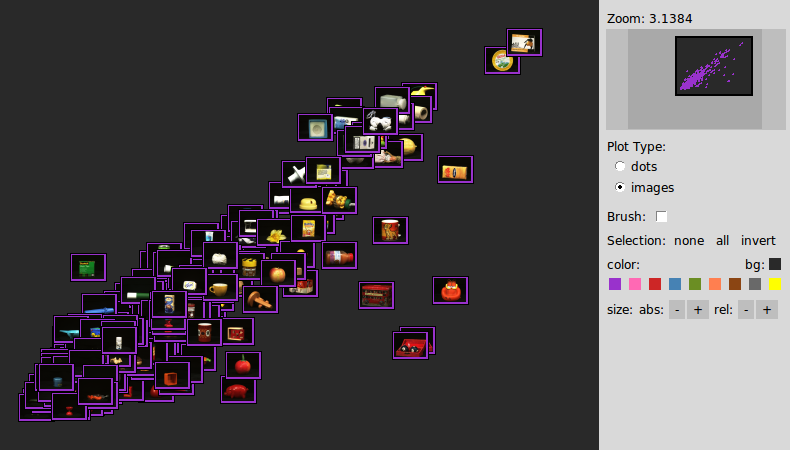
\includegraphics[width = 0.6\textwidth]{img/tk2dImagesObject.png}
\end{center}

  
  
\subsubsection{Working with Star Glyphs}
A star glyph is a visual representation of one data entity. If the entity has p-dimensional data associated, say $x_{i} = (x_{11},x_{12},..., x_{1p})$, the glyph gets constructed as the following graphic outlines:

\begin{center}
  \begin{tikzpicture}
  [dot/.style={shape = circle, fill=black,inner sep = 1pt}]

  \newcommand{\radius}{1}
  \newcommand{\dist}{4}

    \begin{scope}
      \coordinate (x1) at (0:\radius);
      \coordinate (x2) at (72:\radius);
      \coordinate (x3) at (144:\radius);
      \coordinate (x4) at (216:\radius);
      \coordinate (x5) at (288:\radius);

      \draw[->] (0,0) -- (x1) node [right] {$x_1$};
      \draw[->] (0,0) -- (x2) node [ above] {$x_2$};
      \draw[->] (0,0) -- (x3) node [ above] {$x_3$};
      \draw[->] (0,0) -- (x4) node [ left] {$x_4$};
      \draw[->] (0,0) -- (x5) node [ below] {$x_5$};
    \end{scope}

    \begin{scope}[shift={(\dist,0)}]


      \coordinate (x1) at (0:\radius);
      \coordinate (x2) at (72:\radius);
      \coordinate (x3) at (144:\radius);
      \coordinate (x4) at (216:\radius);
      \coordinate (x5) at (288:\radius);

      \draw[->] (0,0) -- (x1) node [right] {$x_1$};
      \draw[->] (0,0) -- (x2) node [ above] {$x_2$};
      \draw[->] (0,0) -- (x3) node [ above] {$x_3$};
      \draw[->] (0,0) -- (x4) node [ left] {$x_4$};
      \draw[->] (0,0) -- (x5) node [ below] {$x_5$};


      \node at ($(0,0)!0.7!(x1)$) [dot] {};
      \node at ($(0,0)!0.3!(x2)$) [dot] {};
      \node at ($(0,0)!0.5!(x3)$) [dot] {};
      \node at ($(0,0)!0.8!(x4)$) [dot] {};
      \node at ($(0,0)!0.6!(x5)$) [dot] {};

    \end{scope}

    \begin{scope}[shift={(2*\dist,0)}]
      \coordinate (x1) at (0:\radius);
      \coordinate (x2) at (72:\radius);
      \coordinate (x3) at (144:\radius);
      \coordinate (x4) at (216:\radius);
      \coordinate (x5) at (288:\radius);

      \fill [fill = yellow!40!orange] ($(0,0)!0.7!(x1)$) -- ($(0,0)!0.3!(x2)$) -- ($(0,0)!0.5!(x3)$) -- ($(0,0)!0.8!(x4)$) -- ($(0,0)!0.6!(x5)$) -- cycle;
      
      
      \draw[->] (0,0) -- (x1) node [right] {$x_1$};
      \draw[->] (0,0) -- (x2) node [ above] {$x_2$};
      \draw[->] (0,0) -- (x3) node [ above] {$x_3$};
      \draw[->] (0,0) -- (x4) node [ left] {$x_4$};
      \draw[->] (0,0) -- (x5) node [ below] {$x_5$};

      \node at ($(0,0)!0.7!(x1)$) [dot] {};
      \node at ($(0,0)!0.3!(x2)$) [dot] {};
      \node at ($(0,0)!0.5!(x3)$) [dot] {};
      \node at ($(0,0)!0.8!(x4)$) [dot] {};
      \node at ($(0,0)!0.6!(x5)$) [dot] {};


    \end{scope}


    \begin{scope}[shift = {(3*\dist,0)}]
      \coordinate (x1) at (0:\radius);
      \coordinate (x2) at (72:\radius);
      \coordinate (x3) at (144:\radius);
      \coordinate (x4) at (216:\radius);
      \coordinate (x5) at (288:\radius);

      \fill [fill = yellow!40!orange] ($(0,0)!0.7!(x1)$) -- ($(0,0)!0.3!(x2)$) -- ($(0,0)!0.5!(x3)$) -- ($(0,0)!0.8!(x4)$) -- ($(0,0)!0.6!(x5)$) -- cycle;

    \end{scope}
   
    
  \end{tikzpicture}
\end{center}

\modify{We decided to use the last image as our star glyph visualization}. We take a look at glyphs using the \texttt{iris} data example. Data and graph object have been defined previous in this vignette. It just stays to define the visualization instructions with the glyph definition

\begin{Schunk}
\begin{Sinput}
> vizGlyph1 <- ng_2d(data = ng.iris, graph = ng.lg, glyph = names(ng.iris)[c(1, 
+     2, 3, 4, 3, 2, 3, 4, 1)])
> vizGlyph2 <- ng_2d(data = ng.iris, graph = ng.lgnot, glyph = shortnames(ng.iris)[c(1, 
+     2, 3, 4, 3, 2, 3, 4, 1)])
> vizGlyph2
\end{Sinput}
\begin{Soutput}
tk2d scatter plot: ng_2d()
Graph: 4D Transition 
Data: iris 
\end{Soutput}
\end{Schunk}
Note that you can either use the \texttt{shortnames} or the \texttt{names} to define the glyph sequence. It stays to call \texttt{navGraph}
\begin{Schunk}
\begin{Sinput}
> nav <- navGraph(ng.iris, list(ng.lg, ng.lgnot), list(vizGlyph1, 
+     vizGlyph2))
\end{Sinput}
\end{Schunk}

\begin{center}
  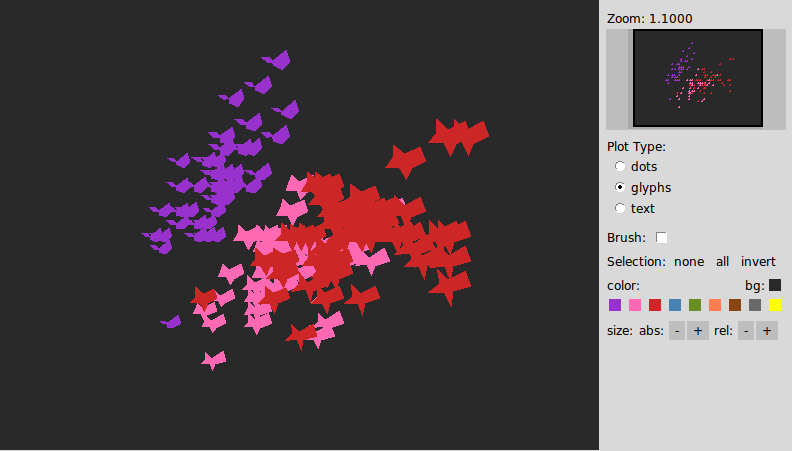
\includegraphics[width = 0.6\textwidth]{img/tk2dGlyphs.png}
\end{center}


\subsubsection{Working with Text}
When defining the \texttt{NG\_data} object, one can specify the \texttt{labels} argument (character) which directly maps to the text radiobutton in the \texttt{tk2d} display.



\subsection{ggobi}
Ggobi allows one to use different elements of data visualization and interaction then the \texttt{tk2d} display (e.g. parallel coordinate plots). Ggobi is superior to the \texttt{tk2d} display if one deals with large data sets. However ggobi does not visualize images nor glyphs. Visualization instructions which address the ggobi device can be created with the \texttt{ng\_2d\_ggobi} command. Let's demonstrate this using the \texttt{iris} data example

\begin{Schunk}
\begin{Sinput}
> vizGgobi1 <- ng_2d_ggobi(data = ng.iris, graph = ng.lg)
> vizGgobi2 <- ng_2d_ggobi(data = ng.iris, graph = ng.lgnot)
\end{Sinput}
\end{Schunk}
and finally start \texttt{navGraph}
\begin{Schunk}
\begin{Sinput}
> nav <- navGraph(ng.iris, list(ng.lg, ng.lgnot), list(vizGgobi1, 
+     vizGgobi2))
\end{Sinput}
\end{Schunk}
or as shown earlier
\begin{Schunk}
\begin{Sinput}
> nav <- navGraph(ng.iris, settings = list(defaultDisplay = "ggobi"))
\end{Sinput}
\end{Schunk}


\subsection{Custom visualization instructions}
%The \texttt{RnavGraph} package allows for additional specific visualization instructions. If you are new to \texttt{navGraph}, you likely should skip this part and move on to the section ``Starting a navGraph Session''. We first initialize the \texttt{iris} data again

\subsubsection{traditional graphic device}
If you want to create your own visualization from scratch instead of using for example the \texttt{tk2d} display, you can define a display function that takes any subset of the following as arguments\\
\begin{center}
 
\begin{tabular}{lp{10cm}}
    \textbf{argument} & \textbf{description}\\ \hline
    x & x-coordinate \\
    y & y-coordinate \\
    group & group slot from \texttt{NG\_data} object\\
    labels & labels slot from \texttt{NG\_data} object\\
    order & order of points. In 3d rigid rotation, the order increases with the distance  of a the point from the viewer.\\
    from & node name the bullet moves from\\
    to & node name the bullet moves to\\
    percentage & in between percentage of bullet\\
    data & data name of \texttt{NG\_data} object  
\end{tabular}
\end{center}

\vspace{1em}
Let's give an example with the traditional graphic device. First of all, a plotting function is needed
\begin{Schunk}
\begin{Sinput}
> myPlot <<- function(x, y, group, labels) {
+     plot(x, y, col = group, pch = 19)
+ }
\end{Sinput}
\end{Schunk}
\modify{note that the order argument only gives an order while the bullet is traversing a 3d rotation (no order at a node).}\\
then, a visualization instruction has to be defined using \texttt{ng\_2d\_myplot}
\begin{Schunk}
\begin{Sinput}
> viz1 <- ng_2d_myplot(ng.iris, ng.lg, fnName = "myPlot", device = "base")
> viz1
\end{Sinput}
\begin{Soutput}
2D Axis Plot: nd_2d_myplot()
Plot function: myPlot 
Graph: 3D Transition 
Data: iris 
\end{Soutput}
\end{Schunk}

and finally, you can call \texttt{navGraph} as used
\begin{Schunk}
\begin{Sinput}
> nav <- navGraph(ng.iris, ng.lg, viz1)
\end{Sinput}
\end{Schunk}
Note, that by default the base graphics system stores all the plotting instructions onto a device in order to be able to redraw the device if it gets moved or scaled etc... In context with \texttt{navGraph} were we are to plot and re-plot the data many times, this behavior is a nuisance and slows down your computer. Hence you can turn this behavior of the current display of (once it exists) with the following command
\begin{Schunk}
\begin{Sinput}
> dev.control(displaylist = "inhibit")
\end{Sinput}
\end{Schunk}

\modify{Note that OSX has a weird implementation of double buffering. You need to let the bullet rest for a while before the display gets refreshed. Hence animations wont work}.\\

Further, see the demos: \texttt{ng\_2d\_myplot\_base} and \texttt{ng\_2d\_myplot\_base}. 

\subsubsection{grid}
See demo: \texttt{ng\_2d\_myplot\_grid}.
\subsubsection{rgl}
See demo: \texttt{ng\_2d\_myplot\_grid}.


\section{Starting a navGraph Session}
\newcommand{\ngwindow}{
\fill [fill=gray!40] (0,0) rectangle (\ww,-0.2);
\fill [fill=brown!10] (0,-0.2) rectangle (\ww,-0.4);
\draw (0,0) rectangle (\ww,-\wh);
\draw (0,-0.2) -- (\ww,-0.2);
\draw (0,-0.4) -- (\ww,-0.4);
}

\newcommand{\nggraph}[9]{
  \begin{scope}[shift= {(2,-3.6/2-0.4)}]
    \node at ( 1, 0)  [#1, label=right:{\scriptsize A:B}] (AB) {};
    \node at ( 0, -1) [#2, label=below:{\scriptsize A:D}] (AD) {};
    \node at (-1, 0)  [#3, label=left:{\scriptsize B:C}] (BC) {};
    \node at ( 0, 1)  [#4, label=above:{\scriptsize C:D}] (CD) {};
    \draw[#5] (AB) -- (AD);
    \draw[#6] (AB) -- (BC);
    \draw[#7] (AB) -- (CD);
    \draw[#8] (AD) -- (BC);
    \draw[#9] (AD) -- (CD);
  \end{scope}
}

\newcommand{\ww}{4}
\newcommand{\wh}{4}

\newcommand{\mouse}[4]{
  \begin{scope}[shift={#1}]
    \filldraw[fill=white, draw = black, line width=1pt] (0,0) -- (-90:0.45) -- (-75:0.35) -- (-70:0.5) -- (-57:0.5) -- (-55:0.35) -- (-40:0.45) -- cycle; 
    \ifthenelse{\equal{#2}{}}{}{\node at #3 [#4, fill=red!30, line width = 1pt, draw = red!50!black, rounded corners] {#2};}
  \end{scope}
}



The \texttt{navGraph} function is the heart of the \texttt{RnavGraph} package. Once the \texttt{NG\_data}, \texttt{NG\_graph} and \texttt{NG\_visualization} objects have been correctly defined, one can pass them to the \texttt{navGraph} function which in turn starts the graphical user interface consisting of the graph with a bullet and the visualizations.\\

We will first discuss the different scenarios the \texttt{navGraph} function accommodates. Then we move on to the graphical user interface description. And finally we show how one can communicate with the graphical user interface from the R prompt via the navGraph handler.

\subsection{Calling navGraph}
The \texttt{navGraph} R function has four arguments: \texttt{data}, \texttt{graph}, \texttt{viz} and \texttt{settings}, where the latter three are optional. Except the \texttt{settings} argument, all of them accommodate either their corresponding \texttt{NG\_} object or a list of their corresponding \texttt{NG\_} objects. A special case poses the \texttt{data} argument which also accepts a navGraph handler in order to continue a saved session. More about that later. There are no constraints about how graphs and data sets are connected via visualization instructions as long they are consistent. For example, say we run $5$ simulations and we would like to compare their results via some visualization with \texttt{navGraph}. Further there might be three graphs we are interested in traversing to explore the difference in the simulation results. This scenario would look like

{\fontsize{11pt}{20pt}
\begin{center}
  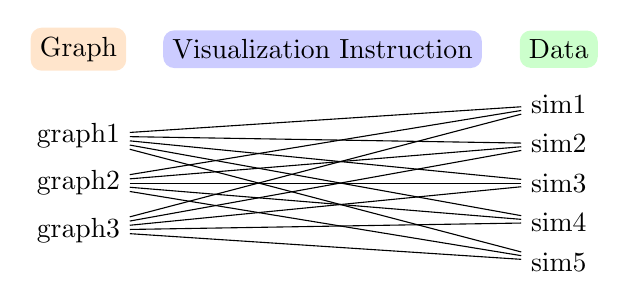
\begin{tikzpicture}
    \node at (6.1,0) [fill=green!20, rounded corners] {Data};
    \node at (3.1,0) [fill=blue!20, rounded corners] {Visualization Instruction};
    \node at (0,0) [fill=orange!20, rounded corners] {Graph};

    \node (s1) at (6.1,-0.7) {sim1};
    \node (s2) at (6.1,-1.2) {sim2};
    \node (s3) at (6.1,-1.7) {sim3};
    \node (s4) at (6.1,-2.2) {sim4};
    \node (s5) at (6.1,-2.7) {sim5};

    \node (g1) at (0,-1.1) {graph1};
    \node (g2) at (0,-1.7) {graph2};
    \node (g3) at (0,-2.3) {graph3};
    
    \foreach \graph in {g1,g2,g3} {
      \foreach \data in {s1,s2,s3,s4,s5} {
        \draw  (\graph) -- (\data);
      }
    }   
  \end{tikzpicture}
\end{center}  
}
where each connecting line represents an \texttt{NG\_visualization} instruction object. One could also only choose a subset of these visualization instructions. Once the graphical user interface is started, the user can then choose the graph he wants to explore and \texttt{navGraph} switches to the visualizations connected to this graph. \modify{Hence, for a single \texttt{navGraph} the user ``looks'' form a single graph perspective at all the data connected via their visualization instructions}. For the iris example we have the following scenario


{\fontsize{11pt}{20pt}
\begin{center}
  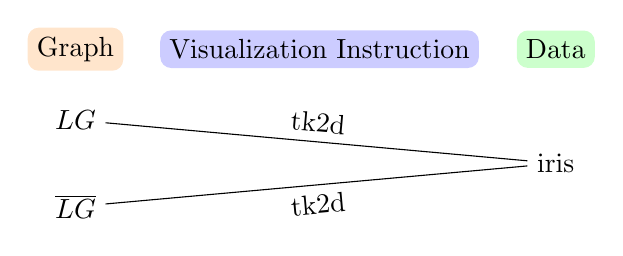
\begin{tikzpicture}
    \node at (6.1,0) [fill=green!20, rounded corners] {Data};
    \node at (3.1,0) [fill=blue!20, rounded corners] {Visualization Instruction};
    \node at (0,0) [fill=orange!20, rounded corners] {Graph};
    
    \node (g1) at (0,-0.9) {$LG$};
    \node (g2) at (0,-2) {$\overline{LG}$};
    
    \node (s1) at (6.1,-1.45) {iris};

    \draw (g1) -- (s1) node [above,midway,sloped] {tk2d};
    \draw (g2) -- (s1) node [below,midway,sloped] {tk2d};
   \end{tikzpicture}
\end{center}  
}

If the \texttt{navGraph} only gets a \texttt{NG\_data}- or a list of \texttt{NG\_data} objects, it creates the graphs and visualization instructions for a 3d and 4d transition graphs connected to the data with the \texttt{tk2d} display.

\subsubsection{Settings}
The \texttt{settings} argument of the \texttt{navGraph} function determines the look and feel of the graph interaction interface. \modify{Currently on can not control the look and feel of the \texttt{tk2d} display}. The \texttt{settings} argument has to be a list optionally containing other named lists. The grand scheme of what can be modified looks like

\begin{center}
\begin{tabular}{|p{4cm}|p{4cm}|p{4cm}|p{4cm}|}
  \hline 
  \textbf{color} (char) & \textbf{interaction} (num) & \textbf{display} & \textbf{tk2d} (num)\\
  \hline
   background       &    bulletRadius          &   NSteps           &   bg (char) \\
   bullet           &    nodeRadius            &   animationTime    &   brush\_colors (vect char)\\
   bulletActive     &    lineWidth             &   dragSelectRadius &    brush\_color (char)\\
   nodes            &    highlightedLineWidth  &   labelDistRadius  &    linked (logical)\\
   nodesActive      &                          &                    &    \\
   adjNodes         &                          &                    &    \\
   adjNodesActive   &                          &                    &    \\
   notVisitedEdge   &                          &                    &    \\
   visitedEdge      &                          &                    &    \\
   edgeActive       &                          &                    &    \\
   labels           &                          &                    &    \\
   labelsActive     &                          &                    &    \\
   adjLabels        &                          &                    &    \\
   adjLabelsActive  &                          &                    &    \\
   path             &                          &                    &    \\
   \hline
\end{tabular}
\end{center}

where the \texttt{color} elements must be character string (recognized as a color) and the \texttt{interaction} and \texttt{display} elements must be numeric. For example the following settings object would work

\begin{Schunk}
\begin{Sinput}
> navGraph(..., settings = list(color = list(background = "green"), 
+     interaction = list(bulletRadius = 4, nodeRadius = 3)))
\end{Sinput}
\end{Schunk}
Note that \modify{everything} is case sensitive according to the table.\\

Additionally, there is an additional option that can be specified in settings. If only a \texttt{NG\_data} object gets passed to \texttt{navGraph} one can choose between the \texttt{tk2d} and \texttt{ggobi} as a display.

\begin{Schunk}
\begin{Sinput}
> navGraph(ng.iris, settings = list(defaultDisplay = "ggobi"))
\end{Sinput}
\end{Schunk}
or 
\begin{Schunk}
\begin{Sinput}
> navGraph(ng.iris, settings = list(defaultDisplay = "tk2d"))
\end{Sinput}
\end{Schunk}
default is the \texttt{tk2d} display.


\subsection{Graphical User Interface}
Once \texttt{navGraph} has initialized the all displays, you will see one window with a graph similar to

\begin{center}
  \begin{tikzpicture}
 [a/.style={circle, draw=black!50, fill=purple!80, minimum size=3mm},
  na/.style={circle, draw=black!50, fill=violet!100, minimum size=3mm},
  bullet/.style={circle, draw=black, fill=yellow!80,thick, minimum size=5mm},
  nc/.style={draw=black!30,line width=1.5pt},
  co/.style={draw=black!30,line width=4pt}]
    \begin{scope}[shift = {(1.5*\ww,0)}]
      \ngwindow
      \nggraph{a}{a}{a}{a}{co}{co}{co}{nc}{nc}
      \node at (AB) [bullet] {};
      \node at (0,-0.7) [right] {0};
    \end{scope}    
  \end{tikzpicture}
\end{center}
and all the data visualization displays connected to the current graph. We will first cover how to interact with the graph display and then move on to the interaction with the \texttt{tk2d} display.\\

Further, in the sections that follow, we will show some stripes of graphics about the interactions. We refer to them via state1, state2, etc... (reset the numbers every time you see new stripe of graphics).


\subsubsection{Move the bullet}
The bullet can be dragged in a intuitive way along the edges of the graph.
{\fontsize{11pt}{20pt}
\begin{center}
  \begin{tikzpicture}
 [a/.style={circle, draw=black!50, fill=purple!80, minimum size=3mm},
  na/.style={circle, draw=black!50, fill=violet!100, minimum size=3mm},
  bullet/.style={circle, draw=black, fill=yellow!80,thick, minimum size=5mm},
  nc/.style={draw=black!30,line width=1.5pt},
  co/.style={draw=black!30,line width=4pt}]
    
    \begin{scope}[shift = {(1.5*\ww,0)}]
      \ngwindow
      \nggraph{a}{na}{na}{a}{nc}{nc}{co}{nc}{nc}
      \node at ($(AB)!0.4!(CD)$) [bullet] {};
      \mouse{($(AB)!0.4!(CD)$)}{}{(-60:0.8)}{right}
      \node at (0,-0.7) [right] {40};
    \end{scope}


    \begin{scope}
      \ngwindow
      \nggraph{a}{a}{a}{a}{co}{co}{co}{nc}{nc}
      \node at (AB) [bullet] {};
      \mouse{(AB)}{Left Click and Drag}{(-120:1)}{right}
      \node at (0,-0.7) [right] {0};
    \end{scope}


    \begin{scope}[shift = {(3*\ww,0)}]
      \ngwindow
      \nggraph{a}{a}{na}{a}{nc}{nc}{co}{nc}{co}
      \draw [co, draw=gray!80!black](AB) -- (CD);
      \node at (CD) [bullet] {};
      \mouse{(CD)}{}{(-60:0.8)}{right}
      \node at (0,-0.7) [right] {0};
    \end{scope}

    
  \end{tikzpicture}
\end{center}
 
}

\begin{enumerate}
\item Bullet on A:B
  \begin{itemize}
  \item All adjoining nodes and their connecting edges are highlighted via line with or color.
  \item The number in the upper left corner indicates the percentage the bullet progressed towards another node
  \end{itemize}
\item Bullet between A:B and C:D
  \begin{itemize}
  \item now only the active edge and nodes are highlighted
  \end{itemize}
\item Bullet arrived on C:D
  \begin{itemize}
  \item Same as in 1) but the edge A:B to C:D has a different color to indicate that we have traversed along this edge.
  \end{itemize}
\end{enumerate}

When you drag the bullet in State 1 towards a node, \texttt{navGraph} won't constrain the bullets move for some small radius around the current node position. This way, as soon as you cross the pre-specified radius, \texttt{navGraph} calculates which edge is closest to the direction you moved the bullet and constrains the bullet to move along this edge. If your graph is so large that it is very hard for you to land on the desired edge, you can also select an adjoining node while in state 1. If the node you select is not adjoining, the bullet jumps to this non adjoining node.

{\fontsize{11pt}{20pt}
\begin{center}
  \begin{tikzpicture}
 [a/.style={circle, draw=black!50, fill=purple!80, minimum size=3mm},
  na/.style={circle, draw=black!50, fill=violet!100, minimum size=3mm},
  bullet/.style={circle, draw=black, fill=yellow!80,thick, minimum size=5mm},
  nc/.style={draw=black!30,line width=1.5pt},
  co/.style={draw=black!30,line width=4pt}]



    
    \begin{scope}[shift = {(3*\ww,0)}]
      \ngwindow
      \nggraph{a}{na}{na}{a}{nc}{nc}{co}{nc}{nc}
      \node at ($(AB)!0.4!(CD)$) [bullet] {};
      \mouse{($(AB)!0.4!(CD)$)}{drag}{(30:0.5)}{right}
      \node at (0,-0.7) [right] {40};
    \end{scope}

    \begin{scope}[shift = {(1.5*\ww,0)}]
      \ngwindow
      \nggraph{na}{na}{na}{a}{nc}{nc}{co}{nc}{nc}
      \node at (AB) [bullet] {};
      \mouse{(CD)}{}{(-60:0.8)}{right}
      \node at (0,-0.7) [right] {0};
    \end{scope}


    \begin{scope}
      \ngwindow
      \nggraph{a}{a}{a}{a}{co}{co}{co}{nc}{nc}
      \node at (AB) [bullet] {};
      \mouse{(CD)}{Select adjoining node}{(-30:0.5)}{right}
      \node at (0,-0.7) [right] {0};
    \end{scope}





    
  \end{tikzpicture}
\end{center}
 
}

Note that once you move along an edge, you can also use your scroll wheel on the mouse to move the bullet. \modify{This is conceptually correct, however \texttt{navGraph} also has an ``active'' (mouse over) node and edge state with a different color. (not shown in the images above).}

\subsubsection{Modify the Graph Layout}
The user can also modify the layout of the graph by dragging nodes on the canvas while pressing the \texttt{CTRL} key.

{\fontsize{11pt}{20pt}
\begin{center}
  \begin{tikzpicture}
 [a/.style={circle, draw=black!50, fill=purple!80, minimum size=3mm},
  na/.style={circle, draw=black!50, fill=violet!100, minimum size=3mm},
  bullet/.style={circle, draw=black, fill=yellow!80,thick, minimum size=5mm},
  nc/.style={draw=black!30,line width=1.5pt},
  co/.style={draw=black!30,line width=4pt}]

    \begin{scope}[shift = {(3*\ww,0)}]
      \ngwindow
      \begin{scope}[shift= {(2,-3.6/2-0.4)}]


      \node at ( 1, 0)  [a, label=right:{\scriptsize A:B}] (AB) {};
      \node at ( 0, -1) [a, label=below:{\scriptsize A:D}] (AD) {};
      \node at (-1, 0)  [a, label=left:{\scriptsize B:C}] (BC) {};
      \node at ( -.5, 1)  [a] (CD) {};
      \draw[co] (AB) -- (AD);
      \draw[co] (AB) -- (BC);
      \draw[co] (AB) -- (CD);
      \draw[nc] (AD) -- (BC);
      \draw[nc] (AD) -- (CD);
      
      \node [circle, fill = blue!20, inner sep=10pt] at (CD) {};      
      \node at (CD)  [a] {};
      
      \node at (-0.8,.7) (CD1) {{\scriptsize C:D}};

    \end{scope}
      \node at (AB) [bullet] {};
      \mouse{(CD1)}{Ctrl \& drag}{(160:0.5)}{left}
      \node at (0,-0.7) [right] {0};
    \end{scope}

    \begin{scope}[shift = {(1.5*\ww,0)}]
      \ngwindow
      \begin{scope}[shift= {(2,-3.6/2-0.4)}]
      \node at ( 1, 0)  [a, label=right:{\scriptsize A:B}] (AB) {};
      \node at ( 0, -1) [a, label=below:{\scriptsize A:D}] (AD) {};
      \node at (-1, 0)  [a, label=left:{\scriptsize B:C}] (BC) {};
      \node at ( -.5, 1)  [a, label=above:{\scriptsize C:D}] (CD) {};
      \draw[co] (AB) -- (AD);
      \draw[co] (AB) -- (BC);
      \draw[co] (AB) -- (CD);
      \draw[nc] (AD) -- (BC);
      \draw[nc] (AD) -- (CD);
    \end{scope}
      \node at (AB) [bullet] {};
      \mouse{(CD)}{drag}{(30:0.5)}{right}
      \node at (0,-0.7) [right] {0};
    \end{scope}


    \begin{scope}
      \ngwindow
      \nggraph{a}{a}{a}{a}{co}{co}{co}{nc}{nc}
      \node at (AB) [bullet] {};
      \node at (0,-0.7) [right] {0};
      \mouse{(CD)}{Ctrl Key \& Left Mouse Button}{(160:2.5)}{right}
    \end{scope}

   
  \end{tikzpicture}
\end{center}
 
}

There are no constraints for the nodes to be moved around \modify{even the canvas border!}. However the labels of the nodes must be moved within the defined \texttt{labelDistRadius} in the interaction settings (colored blue here).

\subsubsection{Animate}
Once you move the bullet on an edge, you can let the bullet move towards one of the two nodes that define the edge by double clicking on that node. If you click on another node, the bullet jumps there. For the case of the bullet being on one node, you can double click on an adjoining node, the first click will act as edge selection and the second click as an animation command. The animation speed is determined by the \texttt{animationTime} variable in the interaction settings. That is, \texttt{animationTime}/\texttt{NSteps} is the pause before the bullet moves an increment towards the node. \modify{Note however that the time from one node to the other is not equal \texttt{animationTime}, since the updating displays and doing other ``housekeeping'' in \texttt{navGraph} also take up time. (More precisely as long as if you select \texttt{animationTime}=0).}

{\fontsize{11pt}{20pt}
\begin{center}
  \begin{tikzpicture}
 [a/.style={circle, draw=black!50, fill=purple!80, minimum size=3mm},
  na/.style={circle, draw=black!50, fill=violet!100, minimum size=3mm},
  bullet/.style={circle, draw=black, fill=yellow!80,thick, minimum size=5mm},
  nc/.style={draw=black!30,line width=1.5pt},
  co/.style={draw=black!30,line width=4pt}]
    
    \begin{scope}[shift = {(1.5*\ww,0)}]
      \ngwindow
      \nggraph{a}{na}{na}{a}{nc}{nc}{co}{nc}{nc}

      \foreach \perc in {0.2,0.4,0.6,0.8} {
        \node at ($(AB)!\perc!(CD)$) [bullet] {};
      }
      \node at (0,-0.7) [right] {40};
    \end{scope}


    \begin{scope}
      \ngwindow
      \nggraph{a}{a}{a}{a}{co}{co}{co}{nc}{nc}
      \node at (AB) [bullet] {};
      \mouse{(CD)}{Double Click}{(-30:0.5)}{right}
      \node at (0,-0.7) [right] {0};
    \end{scope}


    \begin{scope}[shift = {(3*\ww,0)}]
      \ngwindow
      \nggraph{a}{a}{na}{a}{nc}{nc}{co}{nc}{co}
      \draw [co, draw=gray!80!black](AB) -- (CD);
      \node at (CD) [bullet] {};
      \node at (0,-0.7) [right] {0};
    \end{scope}

    
  \end{tikzpicture}
\end{center}
 
}


\subsubsection{Paths}
Instead of guiding the bullet by dragging it along edges, you can also select a path in order to later animate the path (\modify{in the sense of animation above}). You create a path by selecting adjoining nodes while having the shift key pressed down. Once you are done, you can double click on the last node and \texttt{navGraph} will animate \modify{or walk} along the just specified path

{\fontsize{11pt}{20pt}
  \begin{center}
  \begin{tikzpicture}
 [a/.style={circle, draw=black!50, fill=purple!80, minimum size=3mm},
 p/.style={circle, draw=black!50, fill=black, minimum size=3mm},
  na/.style={circle, draw=black!50, fill=violet!100, minimum size=3mm},
  bullet/.style={circle, draw=black, fill=yellow!80,thick, minimum size=5mm},
  pbullet/.style={circle, draw=black, fill=black,thick, minimum size=5mm},
 nc/.style={draw=black!30,line width=1.5pt},
  co/.style={draw=black!30,line width=4pt}]
    

  \begin{scope}
    \ngwindow
    \nggraph{a}{a}{a}{a}{co}{co}{co}{nc}{nc}
    \node at (AB) [bullet] {};
    \node at (0,-0.7) [right] {0};
    \mouse{(CD)}{Shift \& Click}{(160:0.2)}{left}
  \end{scope}
  
  
  \begin{scope}[shift = {(1.1*\ww,0)}]
    \ngwindow
    \nggraph{a}{a}{na}{p}{nc}{nc}{co}{nc}{co}
    \draw [co, draw=black](AB) -- (CD);
    \node at (AB) [pbullet] {};
    \mouse{(AD)}{Shift \& Click}{(160:1.9)}{right}
    \node at (0,-0.7) [right] {0};
  \end{scope}

  \begin{scope}[shift = {(2.2*\ww,0)}]
    \ngwindow
    \nggraph{a}{p}{a}{p}{co}{nc}{nc}{co}{co}
    \draw [co, draw=black](CD) -- (AD);
    \node at (AB) [bullet] {};
    \mouse{(BC)}{Shift \& Double Click}{(130:0.6)}{right}

    \node at (0,-0.7) [right] {0};
  \end{scope}
  
  \begin{scope}[shift = {(3.3*\ww,0)}]
    \ngwindow
      \nggraph{a}{na}{na}{a}{nc}{nc}{co}{nc}{nc}
      
      \foreach \perc in {0.2,0.4,0.6,0.8,1} {
        \node at ($(AB)!\perc!(CD)$) [bullet] {};
      }
      \foreach \perc in {0.2,0.4,0.6,0.8,1} {
        \node at ($(CD)!\perc!(AD)$) [bullet] {};
      }
      \foreach \perc in {0.2,0.4,0.6,0.8,1} {
        \node at ($(AD)!\perc!(BC)$) [bullet] {};
      }
    \end{scope}



    

    
  \end{tikzpicture}
\end{center}
 
}
Note that as soon as you release the shift key, you are \modify{out of the path mode}. However if you go to the Tools > Paths menu on the graph display window, you will find you path as \texttt{Active Path} saved. \modify{The Paths toolbox has some bugs. That is, the scroll bar in the Saved Paths list does not work (if you ever happen to add so many paths). This seems a tk issue, and we plan to address this at a later time point.} The V button stands for ``view path'', the W button for ``walk path'' (animate) \modify{and the R button for record paths you explore while dragging the bullet NOT IMPLEMENTED}.\\

You can also animate a path with the \texttt{ng\_walk} function. The \texttt{ng\_walk} function takes as an argument a navGraph handler and a path either in the form of a vector of node names or in the form of a single string where the sequence of node names is separated by a space. Lets see an example

\begin{Schunk}
\begin{Sinput}
> nav <- navGraph(ng.iris)
> ng_walk(nav, "s.L:s.W s.L:p.L p.L:p.W s.L:p.W")
\end{Sinput}
\end{Schunk}
or the path as a vector
\begin{Schunk}
\begin{Sinput}
> ng_walk(nav, c("s.L:s.W", "s.L:p.L", "p.L:p.W", "s.L:p.W"))
\end{Sinput}
\end{Schunk}
Note that every path sent to \texttt{ng\_walk} gets stored as the active path in the path tool.\\

\modify{Currently, a path is considered to be a sequence of adjoining nodes (no gaps).}

\subsubsection{The navGraph Handler}
The navGraph handler links the graphical user interface with the R prompt. A good example its use was the \texttt{ng\_walk} function we introduced in the last section. The navGraph handler contains all the data, graphs and settings \modify{but not the images} of the \texttt{navGraph} session in progress. Hence if you work with large data, you want to avoid having a many navGraph handlers in your workspace. The navGraph handler gets returned from a \texttt{navGraph} function call
\begin{Schunk}
\begin{Sinput}
> library(RnavGraph)
> ng.iris <- ng_data(name = "iris", data = iris[, 1:4], shortnames = c("s.L", 
+     "s.W", "p.L", "p.W"), group = iris$Species, labels = substr(iris$Species, 
+     1, 2))
> nav <- navGraph(ng.iris)
\end{Sinput}
\begin{Soutput}
Session 1, Data iris is new!
\end{Soutput}
\begin{Sinput}
> nav
\end{Sinput}
\begin{Soutput}
RnavGraph handler:
---
created       : Mon Apr 11 12:47:42 2011 
last updated  : not 
---
graphs        : iris : 3D, iris : 4D 
data          : iris 
\end{Soutput}
\end{Schunk}

You can now brush data and change color and size of objects and add paths. You can save the current state of a \texttt{navGraph} session with \texttt{ng\_update}
\begin{Schunk}
\begin{Sinput}
> nav <- ng_update(nav)
> nav
\end{Sinput}
\begin{Soutput}
RnavGraph handler:
---
created       : Mon Apr 11 12:47:42 2011 
last updated  : Mon Apr 11 12:47:42 2011 
---
graphs        : iris : 3D, iris : 4D 
data          : iris 
\end{Soutput}
\end{Schunk}
Note that the last updated field changed. Updating the navGraph handler is particular useful for getting the new groups (according to color and size of the \texttt{tk2d} or \texttt{ggobi} display).
\begin{Schunk}
\begin{Sinput}
> ng_get(nav)
\end{Sinput}
\begin{Soutput}
possible options are: graphs, paths, data, ggobi, viz
\end{Soutput}
\end{Schunk}
the objects graphs,data and viz are lists of their corresponding \texttt{NG\_object}. However if only one element is in the list, \texttt{ng\_get} unlists the object
\begin{Schunk}
\begin{Sinput}
> ng_get(nav, "data")
\end{Sinput}
\begin{Soutput}
object from NG_data class.
  name: iris 
  data: 150 x 4 
    Variable Names | Short Names
    ----------------------------
    Sepal.Length   | s.L
    Sepal.Width    | s.W
    Petal.Length   | p.L
    Petal.Width    | p.W
  group:  3 groups.
  labels: se, ve, vi. 
\end{Soutput}
\begin{Sinput}
> ng_get(ng_get(nav, "data"), "group")[1:5]
\end{Sinput}
\begin{Soutput}
[1] "cdarkorchid;s5" "cdarkorchid;s5" "cdarkorchid;s5" "cdarkorchid;s5"
[5] "cdarkorchid;s5"
\end{Soutput}
\end{Schunk}
the coding for the \texttt{tk2d} display is ``c<color>;s<size>''. Getting the group for each data point only works with the \texttt{tk2d} and \texttt{ggobi} data display. For any other custom display the user must provide his own way to get the new group classifiers whenever he incorporates a brushing tool. The navGraph handler can also be used to restart a navGraph session
\begin{Schunk}
\begin{Sinput}
> nav1 <- navGraph(nav)
\end{Sinput}
\end{Schunk}
however note that this way the images get lost in the new \texttt{tk2d} display. This is because the images are stored in the \texttt{tcl} layer, and the images are usually too large to be saved in navGraph handlers.\\

Again the example with the \texttt{ng\_walk} function

\begin{Schunk}
\begin{Sinput}
> ng_walk(nav, "s.L:s.W s.L:p.L p.L:p.W s.L:p.W")
> ng_walk(nav, c("s.L:s.W", "s.L:p.L", "p.L:p.W", "s.L:p.W"))
\end{Sinput}
\end{Schunk}

Theoretically, the navGraph handler can be saved using \texttt{save} and restored in a new R session using the \texttt{load} command. However we recommend to initialize a new \texttt{navGraph} session from  scratch if possible.\\

If a \texttt{ggobi} and \texttt{tk2d} display show the same data, then the \texttt{ng\_update} function will ask you whether you want to save the grouping of the \texttt{tk2d} or \texttt{ggobi} display.



\subsection{The \texttt{tk2d} Display}
The \texttt{tk2d} display was programmed by us for the \texttt{RnavGraph} package. It accommodates displaying dots, images, glyphs and text. It also provides the user with a lot of interactivity possibilities such as brushing, zooming and resizing of the window. Further if for a particular graph two \texttt{tk2d} windows display the same data, then the data points are linked between the windows. This means that if you for example change the color and size of some points on one display, the same points in the other window also change color and size.\\


The \texttt{tk2d} window for the iris data looks as follows
\begin{center}
  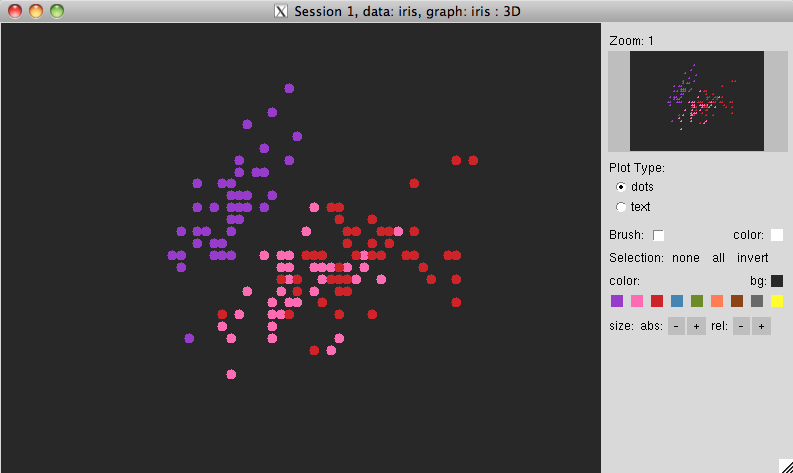
\includegraphics[width = 0.7 \textwidth]{img/Iris2D.png}
\end{center}

The display is designed to be intuitive. So getting familiar with it should not pose any big problems. 

\subsubsection{Zooming and Moving the viewing region}
The \texttt{tk2d} displays the data always twice, in the ``main view'' on the left and in the ``world view'' in the upper right corner. The ``world view'' in the upper right corner always displays all the data points and provides as its name suggest a view of ``your whole data world''. The ``main view'' allows the user to zoom in and out, brush points and deactivate and reactivate points. The zoom factor of the ``main view'' is displayed above the map view. The mouse scroll wheel is used to zoom in and out either while the mouse is placed within the ``world view'' or ``main view''. If the user zooms in or out in the ``main view'' the center of zooming is where the mouse cursor points at, where in the ``world view'' the zooming center is always in the middle of the viewing rectangle. When you zoom in, your current view at the data is shown in the ``world view'' with a rectangle of the same color as background color of the ``main view''.\\

If zoomed in, you can move your current view in the ``main view'' by pressing the right mouse button and dragging your view to the desired place. In the ``world view'' you can just drag and drop the viewing rectangle (left mouse button).
 
 \subsubsection{Brushing and Selecting}
The \texttt{tk2d} display allows to change the color, size and hiding (deactivate) of each object. We use size and color since they are (the only) two attributes that are shared between points, glyphs, images and text. \modify{Currently the text size however does not change!}. You can select points \modify{objects} only in the ``main view'' by either selecting and deselecting them with a left mouse click or by using the brush tool. Selecting them with a mouse click deselects the previously with a mouse click selected point. If you want to select points permanently you need to press the Shift key. When you check the brush checkbox, a gray rectangle appears in the upper right corner. You can resize the brush rectangle by dragging the solid rectangle on its right lower corner. You can move the rectangle by clicking anywhere in the ``main view'' and the brush rectangle jumps to your mouse cursor and also moves with it while your mouse button is still pressed. By default, the points below the brush rectangle don't get brushed permanently. If you want to brush permanently you need to press the Shift key while brushing. Points can only be deselected individually by clicking on them with the shift key pressed, or all together by pressing the non button.

\subsubsection{Deactivating and Reactivating points}
Once you have grouped a set of points by assigning them different color and size, you might want to hide them so you can group the rest of the points without the distraction of the already grouped points. You can do this by selecting these points and then press ``deactivate'' in the modify menu. The button will then stay highlighted to indicate that not all the data is shown. You can deactivate different data points in multiple steps by selecting them and repeatedly pressing the ``deactivate'' button. Once you press the ``reactivate'' button all point will appear again.


 \subsubsection{Changing Color and Size}
Once you have some points selected, you can change their size and color. You can change the size of the points immediately pressing the ``abs'' or ``rel'' + or -. The \texttt{tk2d} gives each object a size attribute. absolute (abs) resizing changes all selected objects to the minimum of the object's sizes plus or minus one size. The relative (rel) resizing increments or decrements all sizes by one. If you were to select five objects with the sizes $\{2,3,3,4,6\}$ and press the rel - button, your new sizes would be $\{1,2,2,3,5\}$ and if you were to press the rel - button again you would get $\{0,1,1,2,5\}$. \modify{Note that you can get negative sizes which theoretically would not show on the ``main view'' anymore, we chose however to display them with minimal possible display size. This might be confusing at the beginning}. If you have a set of points selected with the sizes $\{2,3,3,4,6\}$ and you were to press the abs + button you would get $\{3,3,3,3,3\}$ or the abs - button you would get $\{1,1,1,1,1\}$. Size changes take effect immediately.\\

Changing the color of objects takes place once you have some points brushed and select a colorbox. However you wont notice the change until you deselect all the points. (Use Selection none, invert or all).

\subsubsection{Linking Data between two \texttt{tk2d} displays}
If you display twice (or more) the same data in two \texttt{tk2d} displays that are controlled from within the same or different \texttt{navGraph} sessions, modifying one point in a particular \texttt{tk2d} display modifies all the points from the same data in all \texttt{tk2d} displays. Such an example session could be
\begin{Schunk}
\begin{Sinput}
> V <- shortnames(ng.iris)
> G <- completegraph(V)
> LG <- linegraph(G)
> LGnot <- complement(LG)
> ng.lg <- ng_graph(name = "3D Transition", graph = LG, layout = "circle")
> ng.lgnot <- ng_graph(name = "4D Transition", graph = LGnot, layout = "circle")
> viz1 <- ng_2d(ng.iris, ng.lg, glyphs = V[c(1, 2, 3, 4, 1, 3, 
+     2, 4)])
> viz2 <- ng_2d(ng.iris, ng.lg)
> viz <- list(viz1, viz2)
> graphs <- list(ng.lg, ng.lgnot)
> nav <- navGraph(graph = graphs, data = ng.iris, viz = viz)
\end{Sinput}
\end{Schunk}
Note how \texttt{ng.lg} points twice to the \texttt{ng.iris} data.\\

Alternatively you can also start \texttt{navGraph} twice

\begin{Schunk}
\begin{Sinput}
> nav1 <- navGraph(ng.iris)
> nav2 <- navGraph(ng.iris)
\end{Sinput}
\end{Schunk}
note how a message pops up in the R prompt saying the iris data has been linked. You can tell \texttt{navGraph} that it should not link the data

\begin{Schunk}
\begin{Sinput}
> nav3 <- navGraph(ng.iris, settings = list(tk2d = list(linked = FALSE)))
\end{Sinput}
\end{Schunk}

\modify{Currently, if you wish you had a complete new state, close R and start it again.}


\section{Scagnostics and RnavGraph}
Scagnostics allows one to find graphs that have certain properties, such as the nodes representing clumpy, stringy or convex scatterplots. \modify{Scagnostics is...}. We will demonstrate how you can use scagnostics to the define the variable graphs. The example data in this section is the olive data, provided in the \texttt{RnavGraph} package.
\begin{Schunk}
\begin{Sinput}
> library(scagnostics)
> data(olive)
> ng.olive <- ng_data(name = "Olive", data = olive[, -c(1, 2)], 
+     shortnames = c("p1", "p2", "s", "ol", "l1", "l2", "a", "e"), 
+     group = as.numeric(olive$Area) + 1)
\end{Sinput}
\end{Schunk}
%$
\subsection{The quick way}
The \texttt{scagNav} R function initializes a \texttt{navGraph} session, with 3d and 4d transition graphs that have nodes which satisfy the desired scagnostic property defined with the \texttt{scag} argument. When calling the \texttt{scagnostics} function in the \texttt{scagnostics} R package, \texttt{scagnostics} returns a matrix with all the possible satterplot combinations in the column and all the scagnostic measures in the rows
\begin{Schunk}
\begin{Sinput}
> scagMat <- scagnostics(olive)
> rownames(scagMat)
\end{Sinput}
\begin{Soutput}
[1] "Outlying"  "Skewed"    "Clumpy"    "Sparse"    "Striated"  "Convex"   
[7] "Skinny"    "Stringy"   "Monotonic"
\end{Soutput}
\end{Schunk}

The names of these scagnostic measures in combination with a preceding ``Not'' can be used for the \texttt{scag} argument. If you, for example, look for \texttt{NotClumpy}, a variable $1-Clumpy$ gets generated. Further, you can choose a top fraction of scatterplots showing a certain measure most to be displayed in the graph using the \texttt{topFrac} argument. \texttt{scagNav} will generate for each \texttt{scag} element a 3d and 4d transition graph, except if the \texttt{combineFn} arguments gets specified. The \texttt{combineFn} argument takes any function defined on a vector of scagnostic measure weights such as sum or max. This is for example useful, if you would like to create a graph that either displays clumpy or stringy patterns in its 2d scatterplot nodes.

\begin{Schunk}
\begin{Sinput}
> nav <- scagNav(data = ng.olive, scags = c("Skinny", "Sparse", 
+     "NotConvex"), topFrac = 0.2, combineFn = max, glyphs = shortnames(ng.olive)[1:8], 
+     sep = ":")
\end{Sinput}
\end{Schunk}

or

\begin{Schunk}
\begin{Sinput}
> nav <- scagNav(data = ng.olive, scags = c("Skinny", "Sparse", 
+     "NotConvex"), topFrac = 0.2, glyphs = shortnames(ng.olive)[1:8], 
+     sep = "+")
\end{Sinput}
\end{Schunk}


\modify{Careful, \texttt{scags} is case sensitive.}\\



\subsection{The detailed way}
The \texttt{scagNav} function generates 3d and 4d transition graphs with their corresponding \texttt{tk2d} visualization. We now show how to do each step so that the user can work with the graphs and visualization instructions and finally call the \texttt{navGraph} function. For every \texttt{navGraph} session needs to know the data, graphs and the visualization instruction (this should be your mantra for the next few days). We have already defined the \texttt{ng.olive} data object, we now want to create a variable graph or a set of variable graphs who's edges carry weights from the \texttt{scagnostics} function. Hence we first have to extract the weights of interest. This is done using our \texttt{scagEdgeWeights} function
\begin{Schunk}
\begin{Sinput}
> edgeWts <- scagEdgeWeights(data = ng.olive, scags = c("Clumpy", 
+     "Skinny"))
> edgeWts$fromToEdgeMatrix[1:3, ]
\end{Sinput}
\begin{Soutput}
     from to     Clumpy    Skinny
[1,]    1  2 0.01425229 0.5928461
[2,]    1  3 0.01101357 0.5185595
[3,]    1  4 0.02674608 0.5791038
\end{Soutput}
\begin{Sinput}
> edgeWts$nodeNames
\end{Sinput}
\begin{Soutput}
[1] "p1" "p2" "s"  "ol" "l1" "l2" "a"  "e" 
\end{Soutput}
\end{Schunk}
the numbers in the \texttt{from} and \texttt{to} column correspond with the order of the \texttt{nodeNames}. Note that the \texttt{data} argument can either be a \texttt{NG\_data} object or a \texttt{data.frame}. There is also a \texttt{combineFn} argument which takes a function:
\begin{Schunk}
\begin{Sinput}
> edgeWts <- scagEdgeWeights(data = ng.olive, scags = c("Clumpy", 
+     "Skinny"), combineFn = max)
> edgeWts$fromToEdgeMatrix[1:3, ]
\end{Sinput}
\begin{Soutput}
     from to combined weights
[1,]    1  2        0.5928461
[2,]    1  3        0.5185595
[3,]    1  4        0.5791038
\end{Soutput}
\end{Schunk}
or
\begin{Schunk}
\begin{Sinput}
> edgeWts <- scagEdgeWeights(data = ng.olive, scags = c("Clumpy", 
+     "Skinny"), combineFn = function(x) {
+     2 * x[1] + 3 * x[2]
+ })
> edgeWts$fromToEdgeMatrix[1:3, ]
\end{Sinput}
\begin{Soutput}
     from to combined weights
[1,]    1  2         1.807043
[2,]    1  3         1.577706
[3,]    1  4         1.790803
\end{Soutput}
\end{Schunk}

\modify{Currently, the \texttt{combineFn} only takes a function which returns a single value.}\\

We now could manually create a variable graph using \texttt{newgraph} where we only draw an edge if the \texttt{combined weight} of an edge lies within the top  $20\%$ quantile
\begin{center}
  \setkeys{Gin}{width=0.4\textwidth}
\begin{Schunk}
\begin{Sinput}
> weights <- edgeWts$fromToEdgeMatrix[, "combined weights"]
> ii <- weights > quantile(weights, 0.8)
> G <- newgraph(nodeNames = edgeWts$nodeNames, mat = edgeWts$fromToEdgeMatrix[ii, 
+     c(1, 2)], weights = weights[ii])
> plot(G)
\end{Sinput}
\end{Schunk}
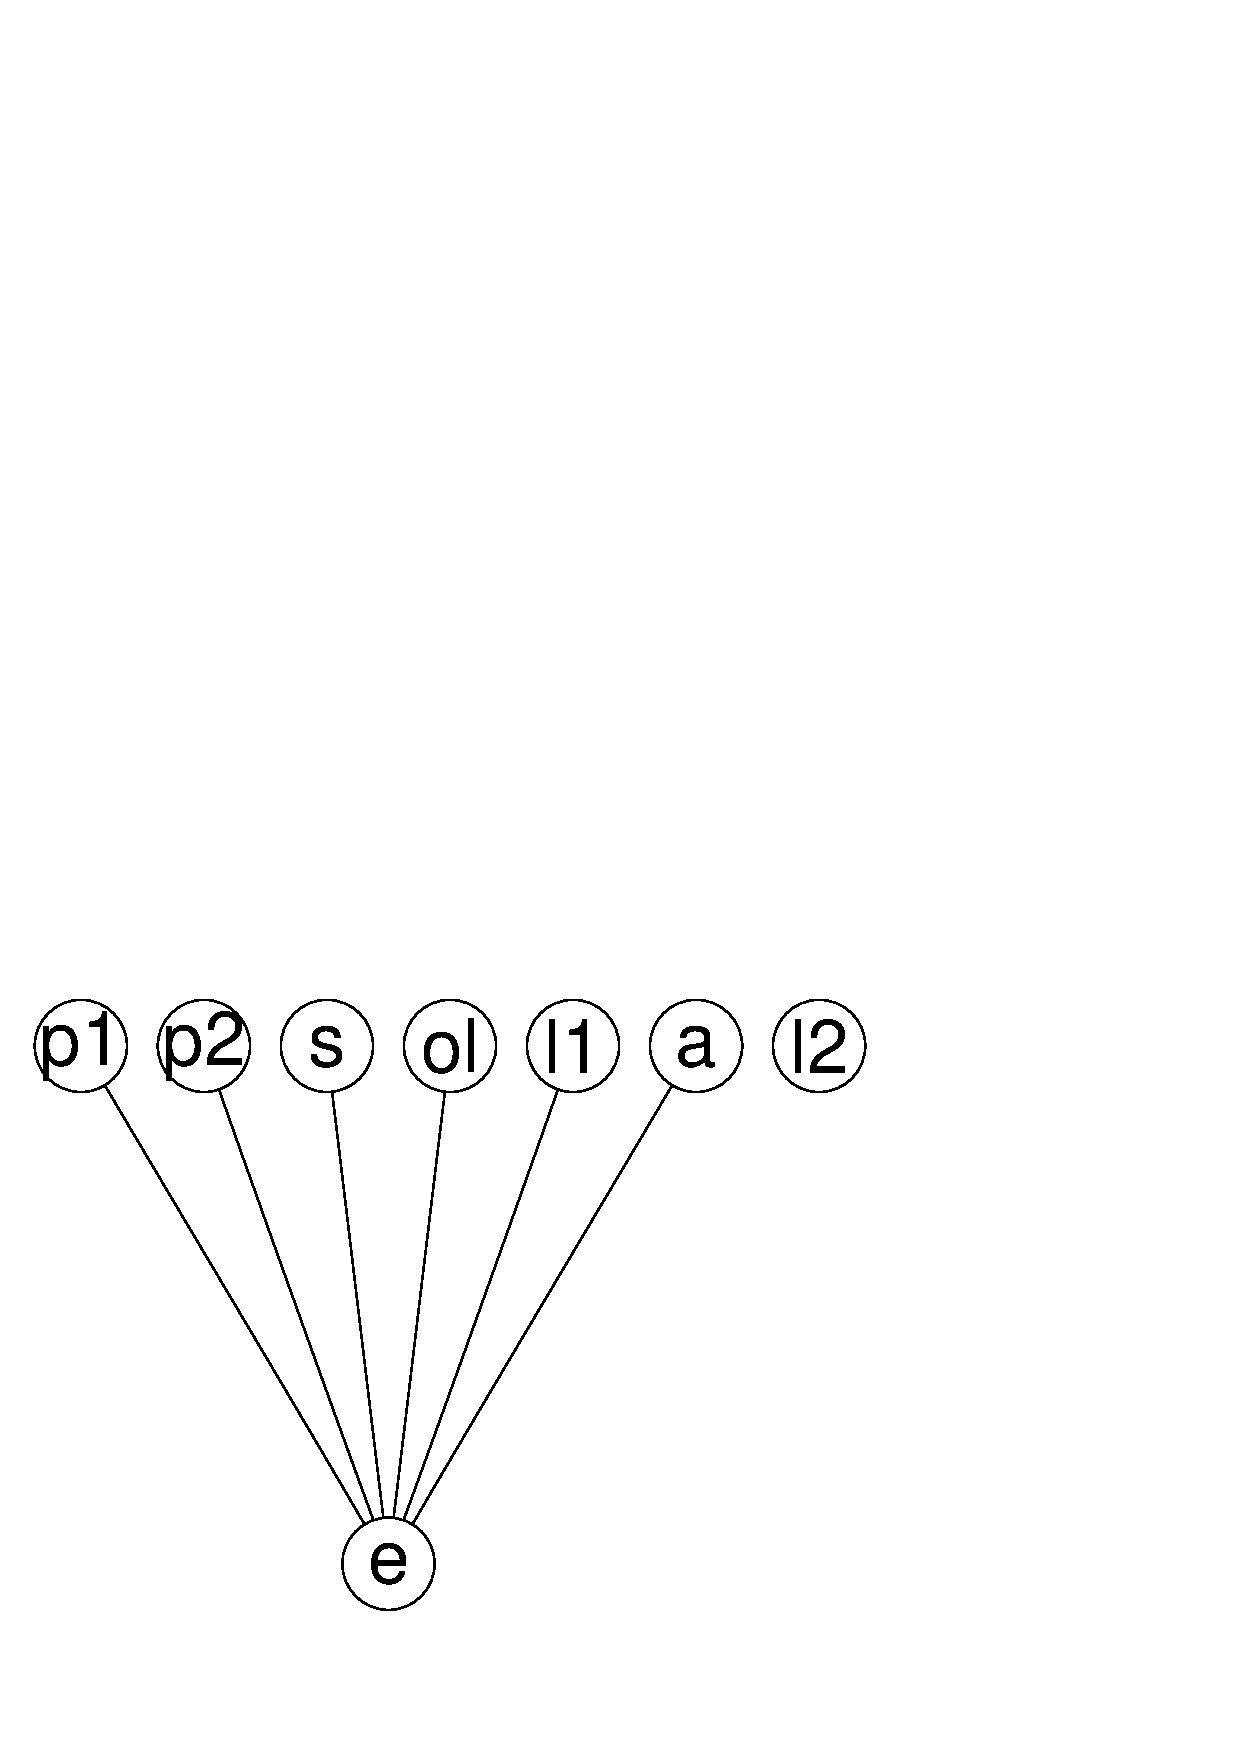
\includegraphics{sweave_p-102}
\end{center}
%$
where the weights are part of the graph \texttt{G}, see for example
\begin{Schunk}
\begin{Sinput}
> edgeData(G, attr = "weight")$"p1|e"
\end{Sinput}
\begin{Soutput}
[1] 2.968342
\end{Soutput}
\end{Schunk}
%$
and hence we could run \texttt{navGraph}
\begin{Schunk}
\begin{Sinput}
> ng.lg <- ng_graph("3d olive", linegraph(G))
> viz <- ng_2d(ng.olive, ng.lg)
\end{Sinput}
\end{Schunk}
\begin{Schunk}
\begin{Sinput}
> nav <- navGraph(ng.olive, ng.lg, viz)
\end{Sinput}
\end{Schunk}

Now this becomes tedious if you have multiple scagnostic measures and hence you would have to create graph for each measure. The \texttt{scagGraph} function simplifies this task. Note how \texttt{scagGraph} creates \texttt{graph} object or a list of \texttt{graph} objects with one single call

\begin{center}
  \setkeys{Gin}{width=0.6\textwidth}
\begin{Schunk}
\begin{Sinput}
> par(mfrow = c(2, 2))
> G_1 <- scagGraph(edgeWts, topFrac = 0.2)
> plot(G_1)
> edgeData(G_1, attr = "weight")$"p1|e"
\end{Sinput}
\begin{Soutput}
[1] 2.968342
\end{Soutput}
\begin{Sinput}
> G_1 <- scagGraph(edgeWts, topFrac = 0)
> plot(G_1)
> G_1 <- scagGraph(edgeWts, topFrac = 1)
> plot(G_1)
> G_1 <- scagGraph(edgeWts, topFrac = 1e-04)
> plot(G_1)
\end{Sinput}
\end{Schunk}
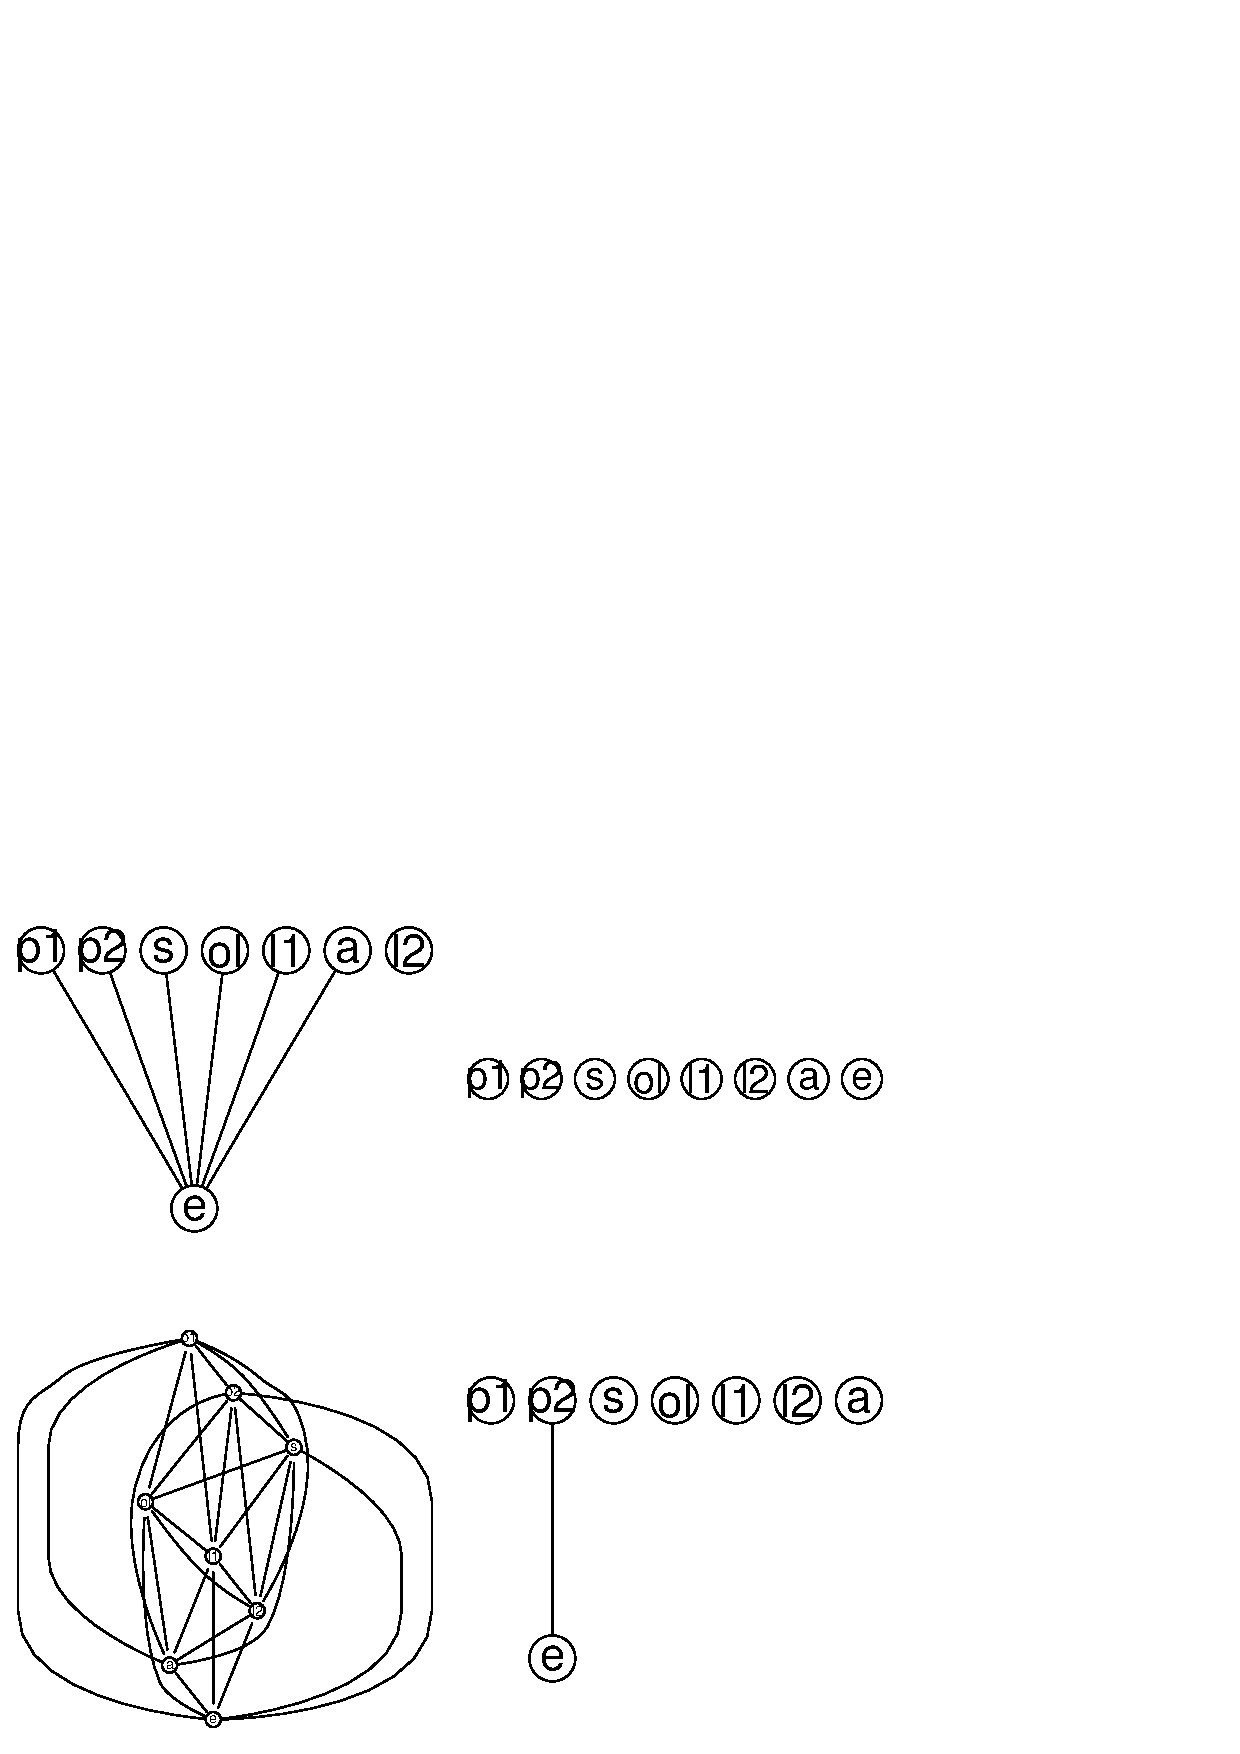
\includegraphics{sweave_p-106}
\end{center}
And for multiple scagnostic measures
\begin{Schunk}
\begin{Sinput}
> edgeWts <- scagEdgeWeights(data = ng.olive, scags = c("Clumpy", 
+     "NotClumpy", "Monotonic"), combineFn = NULL)
> graphList <- scagGraph(edgeWts, topFrac = 0.2)
> graphList
\end{Sinput}
\begin{Soutput}
$Clumpy
A graphNEL graph with undirected edges
Number of Nodes = 8 
Number of Edges = 6 

$NotClumpy
A graphNEL graph with undirected edges
Number of Nodes = 8 
Number of Edges = 6 

$Monotonic
A graphNEL graph with undirected edges
Number of Nodes = 8 
Number of Edges = 6 
\end{Soutput}
\end{Schunk}

Now start \texttt{navGraph}
\begin{Schunk}
\begin{Sinput}
> nav <- navGraph(ng.olive, graphList)
\end{Sinput}
\end{Schunk}
%\modify{Currently only picks up the first graph}.

\section{Example sessions on different data}
In this last section, we will give example code for \texttt{navGraph} sessions using different well known data sets. Some of them are provided by the \texttt{MASS} library

\begin{Schunk}
\begin{Sinput}
> library(MASS)
\end{Sinput}
\end{Schunk}

\subsection{Iris}
\begin{Schunk}
\begin{Sinput}
> ng.iris <- ng_data(name = "iris", data = iris[, 1:4], shortnames = c("s.L", 
+     "s.W", "p.L", "p.W"), group = as.numeric(iris$Species), labels = substr(iris$Species, 
+     1, 2))
> nav <- navGraph(ng.iris)
\end{Sinput}
\end{Schunk}

\subsection{Olive}
\begin{Schunk}
\begin{Sinput}
> library(PairViz)
> data(olive)
> d.olive <- data.frame(olive[, -c(1, 2)])
> ng.olive <- ng_data(name = "Olive", data = d.olive, shortnames = c("p1", 
+     "p2", "s", "oleic", "l1", "l2", "a", "e"), group = as.numeric(olive[, 
+     "Area"]), labels = as.character(olive[, "Area"]))
> ng.olive
> G <- completegraph(shortnames(ng.olive))
> LG <- linegraph(G)
> ng.lg <- ng_graph("3d olive", LG, layout = "kamadaKawaiSpring")
> ng.lgnot <- ng_graph("4d olive", complement(LG), layout = "kamadaKawaiSpring")
> nav <- navGraph(ng.olive, list(ng.lg, ng.lgnot), list(ng_2d(ng.olive, 
+     ng.lg), ng_2d(ng.olive, ng.lgnot)))
> ng_walk(nav, eulerian(as(LG, "graphNEL"))[1:7])
\end{Sinput}
\end{Schunk}

\subsection{US Judge Ratings}
\begin{Schunk}
\begin{Sinput}
> library(MASS)
> ng.data <- ng_data(name = "US Judge Ratings", data = USJudgeRatings)
> p <- ncol(USJudgeRatings)
> adjM <- matrix(0, ncol = p, nrow = p)
> adjM[c(1:8, 11), c(9, 10, 12)] <- 1
> adjM[c(9, 10, 12), c(1:8, 11)] <- 1
> G <- newgraph(names(ng.data), adjM, isAdjacency = TRUE)
> ng.lg <- ng_graph("3d Us Judge", linegraph(G), layout = "fruchtermanReingold")
> nav <- navGraph(ng.data, ng.lg, ng_2d(ng.data, ng.lg))
\end{Sinput}
\end{Schunk}


\subsection{Storm Tracks}
\begin{Schunk}
\begin{Sinput}
> library(rggobi)
> names(stormtracks)
> storms <- stormtracks[, c(2:9, 11)]
> ng.storms <- ng_data(name = "Storm tracks", data = stormtracks[, 
+     c(2:9, 11)], group = as.numeric(stormtracks[, "type"]), labels = stormtracks[, 
+     "type"])
> p <- ncol(ng_get(ng.storms, "data"))
> adjM <- matrix(0, ncol = p, nrow = p)
> adjM[c(1, 2, 4, 5, 6), c(7, 8, 9)] <- 1
> adjM[c(7, 8, 9), c(1, 2, 4, 5, 6)] <- 1
> adjM[c(7, 8, 9), c(7, 8, 9)] <- 1
> adjM[7, 7] <- adjM[8, 8] <- adjM[9, 9] <- 0
> adjM[c(5, 6), c(5, 6)] <- 1
> adjM[5, 5] <- adjM[6, 6] <- 0
> G <- newgraph(names(ng.storms), adjM, isAdjacency = TRUE)
> LG <- linegraph(G)
> ng.lg <- ng_graph("3d storm tracks", LG, layout = "kamadaKawaiSpring")
> ng.lgnot <- ng_graph("4d storm tracks", complement(LG), layout = "kamadaKawaiSpring")
> viz1 <- ng_2d(ng.storms, ng.lg)
> viz2 <- ng_2d(ng.storms, ng.lgnot)
> nav <- navGraph(ng.storms, list(ng.lg, ng.lgnot), list(viz1, 
+     viz2))
\end{Sinput}
\end{Schunk}


\subsection{US cereal}
\begin{Schunk}
\begin{Sinput}
> ng.data <- ng_data(name = "USCereal", data = UScereal[, c(2:8, 
+     10)], shortnames = c("cal", "prot", "fat", "sod", "fib", 
+     "carb", "sug", "pt"), group = UScereal[, 1], labels = UScereal[, 
+     1])
> nav <- navGraph(ng.data)
> nav <- scagNav(ng.data, scags = "Outlying", topFrac = 0.2)
\end{Sinput}
\end{Schunk}

\subsection{Boston Housing}
\begin{Schunk}
\begin{Sinput}
> ng.data <- ng_data(name = "Boston", data = Boston[, -9], shortnames = names(Boston[, 
+     -9]), group = Boston[, "rad"])
> nav <- navGraph(ng.data)
> nav <- scagNav(ng.data, scags = "Clumpy", topFrac = 0.2)
\end{Sinput}
\end{Schunk}

\subsection{Birth Weight}
\begin{Schunk}
\begin{Sinput}
> ng.data <- ng_data(name = "Birth Weight Data", data = birthwt[, 
+     c(1:3, 5:10)], group = birthwt[, 4])
> p <- ncol(ng_get(ng.data, "data"))
> adjM <- matrix(0, ncol = p, nrow = p)
> adjM[c(1:8), c(9)] <- 1
> adjM[c(9), c(1:8)] <- 1
> G <- newgraph(names(ng.data), adjM, isAdjacency = TRUE)
> LG <- linegraph(G, sep = "++")
> ng.lg <- ng_graph("3d birth weight", LG, sep = "++")
> ng.lgnot <- ng_graph("34 birth weight", complement(LG), sep = "++")
> nav <- navGraph(ng.data, list(ng.lg, ng.lgnot), list(ng_2d(ng.data, 
+     ng.lg), ng_2d(ng.data, ng.lgnot)))
\end{Sinput}
\end{Schunk}

\subsection{Swiss bank note data}
\begin{Schunk}
\begin{Sinput}
> require(alr3)
> data(banknote)
> names(banknote[, 1:6])
> ng.data <- ng_data(name = "Swiss bank note Data", data = banknote[, 
+     1:6], shortnames = names(banknote[, 1:6]), group = banknote[, 
+     7])
> nav <- navGraph(ng.data)
> nav <- scagNav(ng.data, scags = "Clumpy", topFrac = 0.2)
\end{Sinput}
\end{Schunk}

\subsection{Body Dimensions Data}
\begin{Schunk}
\begin{Sinput}
> require(gclus)
> data(body)
> names(body[, 1:10])
> ng.data <- ng_data(name = "Body Dimensions", data = body[, 1:24], 
+     group = body[, 25])
> nav <- navGraph(ng.data)
> nav <- scagNav(ng.data, scags = "Clumpy", topFrac = 0.1)
\end{Sinput}
\end{Schunk}

\subsection{Ozone Data}
\begin{Schunk}
\begin{Sinput}
> require(gclus)
> data(ozone)
> ng.data <- ng_data(name = "Ozone data", data = ozone)
> nav <- navGraph(ng.data)
> p <- ncol(ng_get(ng.data, "data"))
> adjM <- matrix(0, ncol = p, nrow = p)
> adjM[c(1), c(2, 4, 5, 6)] <- 1
> adjM[c(2, 4, 5, 6), c(1)] <- 1
> G <- newgraph(names(ng.data), adjM, isAdjacency = TRUE)
> LG <- linegraph(G)
> ng.lg <- ng_graph("3d ozone", LG, layout = "circle")
> ng.lgnot <- ng_graph("4d ozone", complement(LG), layout = "circle")
> nav <- navGraph(ng.data, list(ng.lg, ng.lgnot), list(ng_2d(ng.data, 
+     ng.lg), ng_2d(ng.data, ng.lgnot)))
\end{Sinput}
\end{Schunk}

\subsection{Swiss fertility}
\begin{Schunk}
\begin{Sinput}
> ng.data <- ng_data(name = "SwissFertility", data = swiss, shortnames = c("Fer", 
+     "Agri", "Exam", "Edu", "Cath", "IM"))
> p <- ncol(swiss)
> adjM <- matrix(0, ncol = p, nrow = p)
> adjM[1:5, 6] <- 1
> adjM[6, 1:5] <- 1
> G <- newgraph(shortnames(ng.data), adjM, isAdjacency = TRUE)
> LG <- linegraph(G)
> ng.lg <- ng_graph("3d fertility", LG, layout = "circle")
> ng.lgnot <- ng_graph("4d fertility", complement(LG), layout = "fruchtermanReingold")
> nav <- navGraph(ng.data, list(ng.lg, ng.lgnot), list(ng_2d(ng.data, 
+     ng.lg), ng_2d(ng.data, ng.lgnot)))
\end{Sinput}
\end{Schunk}

\subsection{Challenger}
\begin{Schunk}
\begin{Sinput}
> require(alr3)
> data(challeng)
> ng.data <- ng_data(name = "Challenger Data", data = challeng[, 
+     c(1:3, 5:7)])
> p <- ncol(ng_get(ng.data, "data"))
> adjM <- matrix(0, ncol = p, nrow = p)
> adjM[c(1, 2), c(3:6)] <- 1
> adjM[c(3:6), c(1, 2)] <- 1
> G <- newgraph(names(ng.data), adjM, isAdjacency = TRUE)
> LG <- linegraph(G)
> ng.lg <- ng_graph("3d challenger", LG)
> ng.lgnot <- ng_graph("4d challenger", complement(LG))
> nav <- navGraph(ng.data, list(ng.lg, ng.lgnot), list(ng_2d(ng.data, 
+     ng.lg), ng_2d(ng.data, ng.lgnot)))
\end{Sinput}
\end{Schunk}

\subsection{Animal}
\begin{Schunk}
\begin{Sinput}
> library(PairViz)
> require(cluster)
> data(animals)
> names(animals)
> ng.data <- ng_data(name = "Animal Data", data = animals)
> nav <- navGraph(ng.data)
> ng_walk(nav, eulerian(as(ng_get(ng_get(nav, "graphs")[[1]], "graph")), 
+     "graphNEL"))
\end{Sinput}
\end{Schunk}


\section*{References}

\begin{itemize}

\item Hurley, C. and R.W. Oldford (2011), 
 ``Graphs as navigational infrastructure for high dimensional data spaces'',  ({\it Computational Statistics}, to appear).


\end{itemize}
\end{document}
